%This template was prepared by Dorothea F. Brosius of the 
%Institute for Electronics and Applied Physics, University of Maryland, College Park, MD
%The template was last updated in March 2013
%Thesis Main Page used with thesis.sty based on the
%University of Maryland Electronic Thesis and Dissertation (ETD) Style Guide

\documentclass[12pt]{thesis}  %12pt is larger than 11pt
%\usepackage[pctex32]{graphics}
\usepackage{titlesec}
   \titleformat{\chapter}
      {\normalfont\large}{Chapter \thechapter:}{1em}{}
 
\usepackage{graphicx}
\usepackage{cite}
\usepackage{lscape}
\usepackage{indentfirst}
\usepackage{latexsym}
\usepackage{multirow}
\usepackage{tabls}
\usepackage{wrapfig}
\usepackage{slashbox}
\usepackage{longtable}
\usepackage{subfigure}

\usepackage{amsmath}
\usepackage{algorithmic}

\newcommand{\tbsp}{\rule{0pt}{18pt}} %used to get a vertical distance after \hline
\renewcommand{\baselinestretch}{2}
\setlength{\textwidth}{5.9in}
\setlength{\textheight}{9in}
\setlength{\topmargin}{-.50in}
%\setlength{\topmargin}{0in}    %use this setting if the printer makes the the top margin 1/2 inch instead of 1 inch
\setlength{\oddsidemargin}{.55in}
\setlength{\parindent}{.4in}
\pagestyle{empty}

\begin{document}

%Abstract Page 

\hbox{\ }

\renewcommand{\baselinestretch}{1}
\small \normalsize

\begin{center}
\large{{ABSTRACT}} 

\vspace{3em} 

\end{center}
\hspace{-.15in}
\begin{tabular}{ll}
Title of dissertation:    & {\large A Search for the Neutrinoless Double Beta Decay}\\
&                           {\large of Xenon-136 with Improved} \\
&                           {\large Sensitivity from Waveform Denoising} \\
\ \\
&                          {\large  Clayton G. Davis, Doctor of Philosophy, 2014} \\
\ \\
Dissertation directed by: & {\large  Professor Carter Hall} \\
&  				{\large	 Department of Physics } \\
\end{tabular}

\vspace{3em}

\renewcommand{\baselinestretch}{2}
\large \normalsize

\singlespace{
The EXO-200 detector is designed to search for a theorized decay process of xenon-136 called neutrinoless double-beta ($\beta\beta 0\nu$) decay.  $\beta\beta 0\nu$ decay, if it occurs, would have important consequences for our understanding of the neutrino sector of the standard model.  It would demonstrate the type of the neutrino mass term; set the mass scale of the neutrino sector; and demonstrate the first direct observation of lepton number non-conservation.  The $\beta\beta 0\nu$ decay produces a monoenergetic peak, so one important approach to reducing backgrounds for this search is by improving the energy resolution of the detector.

The present work describes a new analysis technique which improves resolution in the scintillation channel by a combination of waveform denoising and weighting of waveform components based on their expected signal-to-noise ratio; the overall resolution of the detector is improved by better than $20\%$.  Application of this method results in a halflife limit on $\beta\beta 0\nu$ decay in xenon-136 of $T_{1/2} > 1.1 \cdot 10^{25}$ years at $90\%$ confidence.  Further improvements which could impact the energy resolution of EXO-200 are also described, and implications for the planned nEXO experiment are considered.
}
 %(must be first, required, non-numbered)
%Titlepage

\thispagestyle{empty}
\hbox{\ }
\vspace{1in}
\renewcommand{\baselinestretch}{1}
\small\normalsize
\begin{center}

\large{{SIGNAL DENOISING FOR EXO-200 AND AN IMPROVED LIMIT ON NEUTRINOLESS DOUBLE-BETA DECAY}}\\
\ \\
\ \\
\large{by} \\
\ \\
\large{Clayton G. Davis}%Your full name as it appears in University records.
\ \\
\ \\
\ \\
\ \\
\normalsize
Dissertation submitted to the Faculty of the Graduate School of the \\
University of Maryland, College Park in partial fulfillment \\
of the requirements for the degree of \\
Doctor of Philosophy \\
2014
\end{center}

\vspace{7.5em}

\noindent Advisory Committee: \\
Professor Carter Hall, Chair/Advisor \\
Professor Radu Balan \\
Professor Betsy Beise \\
Professor Rabindra Mohapatra \\
Professor Peter Shawhan
 %(must follow Abstract, required, non-numbered)
%Copyright

\thispagestyle{empty}
\hbox{\ }

\vfill
\renewcommand{\baselinestretch}{1}
\small\normalsize

\vspace{-.65in}

\begin{center}
\large{\copyright \hbox{ }Copyright by\\
Clayton Davis  %Type your name as it appears in University records
\\
2014}
\end{center}

\vfill
 %(highly recommended, non-numbered)

%Pages from this point start at lower-case Roman number ii)
\pagestyle{plain}
\pagenumbering{roman}
\setcounter{page}{2}

%Preface

\renewcommand{\baselinestretch}{2}
\small\normalsize
\hbox{\ }
 
\vspace{-.65in}

\begin{center}
\large{Preface} 
\end{center} 


If needed.
  %(if present, start at lower-case Roman number ii)
%Foreword

\renewcommand{\baselinestretch}{2}
\small\normalsize
\hbox{\ }
 
\vspace{-.65in}

\begin{center}
\large{Foreword} 
\end{center} 

If needed.
 %(if present, lower-case Roman)
%Dedication

\renewcommand{\baselinestretch}{2}
\small\normalsize
\hbox{\ }
 
\vspace{-.65in}

\begin{center}
\large{Dedication}
\end{center} 

If needed.
 %(if present, lower-case Roman)
%Acknowledgments

\renewcommand{\baselinestretch}{2}
\small\normalsize
\hbox{\ }
 
\vspace{-.65in}

\begin{center}
\large{Acknowledgments} 
\end{center} 

\vspace{1ex}

Without the help of my colleagues, advisor, friends, family, and my wife, this thesis and the work it embodies would never have happened.  I would like to give thanks to the EXO-200 collaboration, which has provided a supportive and stimulating environment for my work and learning over the past four years.

Particular thanks must go to: David Auty, Phil Barbeau, Giorgio Gratta, Steve Herrin, Sam Homiller, Mike Jewell, Tessa Johnson, Tony Johnson, Caio Licciardi, Mike Marino, Dave Moore, Russell Neilson, Igor Ostrovskiy, J.J. Russell, Kevin O'Sullivan, Tony Waite, Josiah Walton, Liangjian Wen, Liang Yang, and of course my advisor Carter Hall.  I can honestly say that each one of you directly made the following work possible with your contribution of insight, data, plots, and analysis.  Denoising has been a tremendously collaborative effort, and I am grateful that my last project with this group has provided the chance to work with all of you so closely.
 %(if present, lower-case Roman)

\renewcommand{\baselinestretch}{1}
\small\normalsize
\tableofcontents %(required, lower-case Roman)
\newpage
%\listoftables %(if present, lower-case Roman)
%\newpage
\listoffigures %(if present, lower-case Roman)
\newpage
% LIST OF ABBREVIATIONS
\addcontentsline{toc}{chapter}{List of Abbreviations}
%List of Abbreviations

\renewcommand{\baselinestretch}{1}
\small\normalsize
\hbox{\ }

\vspace{-4em}

\begin{center}
\large{List of Abbreviations}
\end{center} 

\vspace{3pt}

\begin{tabular}{ll}
EXO & Enriched Xenon Observatory \\
APD & Avalanche Photo-diode \\
\end{tabular}


\newpage
\setlength{\parskip}{0em}
\renewcommand{\baselinestretch}{2}
\small\normalsize

%Pages from this point start at Arabic numeral 1
\setcounter{page}{1}
\pagenumbering{arabic}
\renewcommand{\thechapter}{6}
\chapter{The Lightmap}
\label{ch:Lightmap}

EXO-200 uses a lightmap to characterize the expected scintillation pulse magnitudes from scintillation clusters with a known position and energy.  Chapter~\ref{ch:DenoisingResults} has shown that the lightmap is a critical input to the denoising algorithm.  In this chapter, we develop from a simpler type of lightmap used in prior analysis to a fully detailed individual-APD lightmap which characterizes scintillation pulse magnitudes on every channel as they depend on scintillation cluster position.  All of this is done in a time-dependent fashion, so the main result of this chapter will be, for each APD channel, a four-dimensional function of scintillation cluster position and time that yields the expected pulse magnitudes.  In section~\ref{sec:LightmapHistory} we describe the lightmap which existed prior to this work, its accomplishments, and its issues which made an upgrade necessary.  Section~\ref{sec:FourDimLightmapParent} will present details of the production of the lightmap from empirical data; deviations from that algorithm for the present analysis are presented in section~\ref{sec:LightmapImplementationDetails}.  Visualizations of the result are provided in section~\ref{sec:LightmapVisualization}.

\section{A History of EXO-200 Lightmaps}\label{sec:LightmapHistory}

The EXO-200 detector has roughly 450 APDs ganged into 74 data channels of five to seven APDs each. Three of the APD ganged channels were disabled due to noisy components before physics data collection began; a fourth channel was disabled in February 2012 due to increasing noise.  The APDs are set into the two endcaps of the cylindrical EXO-200 detector.  To improve light collection, teflon sheets cover the inside of the detector and reflect light back into the liquid xenon rather than allowing it to be absorbed by the vessel walls.

Scintillation is not collected uniformly by all APDs.  Given the same amount of energy deposited into the detector, APDs channels nearest to the deposited energy show significantly larger pulses than APD channels far from the deposit.   To accurately measure the true scintillation energy, it is critical to map out the response of the APDs as a function of deposit position $\vec{x}$.

Furthermore, the APDs and their front-end electronics show time-dependent changes. Gains drift in each APD channel at a variety rates, and stepwise changes occur when the electronics are changed or channels are disabled. This has happened on multiple occasions during the course of the experiment.  This means that, in addition to mapping the response of the APDs as a function of deposit position $\vec{x}$, we must also map it as a function of  time. We call this the lightmap.

Earlier lightmaps were derived from periodic source calibration campaigns collected over one or more days. The ``strong'' Thorium-228 source ($34.04$ kBq, or 0.9201 $\mu$Ci, on September 1, 2009~\cite{SourceCertificates}) was used, and an on-site expert would  position the source in a wide range of locations around the detector.  The $2615$-keV single-site gamma line of the Thallium-208 (a daughter product of Thorium-228) allows the pulse magnitude from a single-position mono-energetic deposit in the detector to be determined in offline analysis.

Even with such a significant quantity of source data, statistics are generally insufficient to fully characterize the lightmap with this method.  The source guide tube shown in figure~\ref{fig:CalibrationGuideTube} does not approach near to every region of the detector; as a result, some regions are difficult to illuminate with the 2615 keV gamma line.  Additionally, APD pulses on individual channels may be quite small for cluster positions which are not quite near to the APDs, compounding the problem of low statistics.  To simplify the problem, pulses on the waveforms of each endcap can be summed together (without gain corrections) such that the 70 or 71 active APD channels can be treated as merely two APD sum channels.  This effectively increases the size of the pulses and the signal-to-noise ratio of these waveforms. It also makes the spatial dependence of the response smoother, so that a coarser binning of the position coordinates is sufficient to characterize the response.  The resulting lightmap was characterized in~\cite{ThesisSteve} and used in~\cite{bb0nSearch2012,bb2nEXO2014} to perform a precision measurement of the rate of $\beta\beta 2\nu$ decay and a search for $\beta\beta 0\nu$ decay in $^{136}$Xe.

Although this lightmap produced significant improvements in the energy resolution achieved by the EXO detector,  it is an incomplete characterization of the APD response.  For example, for $\beta\beta0\nu$ studies we place a fiducial volume cut as close to the edges of the detector as possible, and in certain regions of the detector the scintillation pulse is highly concentrated on a small number of channels.  Summing together multiple channels is, in this case, a lossy form of compression of the data, and it is possible to extract a better energy measurement if it is avoided.

\begin{table}
\begin{center}
\begin{tabular}{|c|c|r|}
\hline Nominal Source Position & Deployment Position & Triggers \\
\hline P2\_nz & S2 & 6207613 \\
P4\_px & S5 & 85931937 \\
P2\_pz & S8 & 5395820 \\
P4\_py & S11 & 6775279 \\
P4\_ny & S17 & 5482649 \\
Other & Other & 1773128 \\ \hline
\end{tabular}
\end{center}
\caption{The total number of thorium triggers taken at each source position; data include only runs which were used to generate the lightmap.  Nominal source position follows a code where the number is 2 for anode runs and 4 for cathode runs; the second part of the code indicates the non-zero coordinate, eg. `px' means positive-x direction, `nz' means negative-z direction.  A diagram of the source tube is shown in figure~\ref{fig:CalibrationGuideTube}.}
\label{tab:TriggerStatsBySourcePos}
\end{table}

The present chapter addresses the challenges inherent with the formulation of an individual-APD lightmap.  We do this primarily by a significant increase in available statistics: whereas the older lightmap used thorium data from a specific calibration campaign lasting for only a few days, we combine all thorium data that has ever been collected by the EXO-200 detector between October 5, 2011 and June 24, 2013.  The total number of triggers included in this dataset are listed in table~\ref{tab:TriggerStatsBySourcePos}.  This vast extension of the available data raises the challenge that APD behavior is time-dependent, so pulse magnitudes may not be constant throughout the dataset; we account for this with a parametrization of the lightmap which permits us to simultaneously extract this time-dependent behavior and the position-dependent light yield that is independent of time.  The result is a complete characterization of light yield in EXO-200.

The denoising algorithm described in chapter~\ref{ch:DenoisingTheory} describes one analysis by which we can exploit knowledge of the behavior of individual APD channels; other analyses include reducing our scintillation thresholds by allowing us to search for pulses in subsets of the APDs rather than only in sums across entire endcaps.  Thus, characterizing the APD yield on individual APD-gang channels is a key component of denoising and may enable additional future studies which would benefit from individual APD channel information.  Section~\ref{sec:FourDimLightmapParent} describes the method used to extract an individual-APD lightmap.

\section{Four-Dimensional Lightmap}\label{sec:FourDimLightmapParent}

As described above, in constructing a channel-by-channel lightmap we face two conflicting needs: we must use as much data as possible to handle the rapid spatial variation and smaller pulses which are expected, but if too much data is included then we run the risk of combining data taken when an APD or the electronics had a different gain.  If we truly wish to use all available data, then we must simultaneously understand the full time-dependence of the gain.  In other words, rather than forming a small number of independently-measured three-dimensional lightmaps, we instead measure a four-dimensional lightmap $L(\vec{x},t)$.  Since we use Thorium-228 source data to generate the lightmap, we require that our lightmap should predict the magnitude of the pulses on each APD gang induced by a single-site deposit of energy $2615$ keV.  Figure~\ref{fig:SampleAPDTemplates} shows our definition of a unit-magnitude pulse.

This may at first seem infeasible.  After all, adding an extra time dimension to the arguments of the lightmap is equivalent to generating a new lightmap for every time bin, which is exactly the situation we wish to avoid.  But we can make a simplifying assumption that the lightmap is separable.  In a physical sense, we assume that:
\begin{enumerate}
\item From a given position $\vec{x}$, photons deposit on each APD channel at a constant rate.
\item Each APD channel amplifies and shapes its pulse with a gain which may vary in time, but does not depend on the point of origin of the photons.
\end{enumerate}
So, we demand that the lightmap have the much simpler form
\begin{equation} \label{eqn:SeparableLightmap}
L(\vec{x},t) = R(\vec{x})S(t)
\end{equation}

Although this is a reasonable approximation, there are details which are omited by this model.  Since the electric field and the reflectivity of detector surfaces are constant in time, assumption 1 is likely to be valid.

However, assumption 2 may not hold in certain cases. For example, each channel draws its pulse from multiple APDs, each of which has an independent time-varying gain.  Photons from a deposit may preferentially sample the gain from the closest APD within a channel, so deposits in different locations may track more closely the gain of the closest APD within a channel.  A study of the impact of this effect is a topic for future study. The analysis presented here will treat it as a small effect.

One simple scheme to find $R$ and $S$ iteratively is described in algorithm~\ref{alg:LightmapScheme}.  Step~\ref{algline:LightmapFormListOfHits} of that algorithm is to select $2615$-keV single-site events; it is understood that some compton-scattered events will inevitably leak into our selection window, but we use the best available energy measurements to minimize that likelihood. As analysis improvements continue to improve the energy resolution, the number of selected compton-scattered events will become smaller and the quality of the lightmap will improve.  The rest of the algorithm describes how we can efficiently converge on estimates of $R(\vec{x})$ and $S(t)$ through an iterative approach.  We do not prove that the algorithm is guaranteed to converge; however, in practice $S(t)$ is almost constant, resulting in fairly rapid convergence.

\begin{algorithm}
\caption{Generating a Lightmap}
\label{alg:LightmapScheme}
\algsetup{indent=2em} % Recommended by the package authors; the default is only for backward compatibility.
\begin{algorithmic}[1]
\STATE Tabulate, using the best energy measurement available, a list of single-site 2615-keV events from Thorium-228 source data. \label{algline:LightmapFormListOfHits}
\STATE Set $S(t) = 1$ for all APD channels.
\REPEAT
  \STATE For each APD channel, estimate $R(\vec{x}) = L(\vec{x},t)/S(t)$ from the set of events tabulated in line ~\ref{algline:LightmapFormListOfHits}.
  \STATE For each APD channel, estimate $S(t) = L(\vec{x},t)/R(\vec{x})$ from the set of events tabulated in line ~\ref{algline:LightmapFormListOfHits}.
\UNTIL convergence is reached.
\end{algorithmic}
\end{algorithm}


\section{Algorithm Details}

The previous section outlines a general algorithm for computing a four-dimensional channel-by-channel lightmap from source data.  In this section we specify the implementation choices which are made in the code currently in use by EXO-200.  In attempt to encourage future experimentation, alternative options will also be listed in some detail, along with some motivations for these alternatives.  Time has not permitted testing of all of these options, but it is hoped that they will be explored in the future.

\subsection{Event Selection}\label{sec:LightmapEventSelection}

The single-site Thorium-228 spectrum is well-peaked at 2615 keV, making it an excellent monoenergetic calibration line.  Our challenge is to select truly 2615-keV events as efficiently as possible, while simultaneously avoiding near-2615-keV events which may leak into the dataset.

This is inherently an iterative process.  The first lightmap is constructed from events selected based on an ionization-only spectrum because no useful position-corrected scintillation measurement yet exists. The resolution of the ionization-only spectrum is relatively poor, roughly $3.5\%$ (sigma) of the energy, as described in \cite{ThesisSteve}, and compromises are made to keep the Compton-shoulder leakage to acceptable levels.  \cite{ThesisSteve} required events to have ionization between $+0.33\sigma$ and $+3\sigma$ of the ionization peak.

Such a strongly asymmetric cut is chosen to avoid leakage from compton shoulder events.  However, because of the anticorrelation between scintillation and ionization, events whose ionization fluctuates high preferrentially selects events whose scintillation fluctuates low, introducing a bias in the pulse magnitude.  Additionally, the cut accepts less than $37\%$ of good events, which is a substantial loss of event statistics. This has a significant impact in certain low-statistics regions of the detector.

The current work benefits from this existing position-corrected scintillation measurement of \cite{ThesisSteve}, leading to a rotated energy spectrum with resolution of roughly $1.8\%$.  As a result, it is possible to accept more events while still keeping Compton shoulder leakage small.  We currently accept events within $2\sigma$ of the peak, with better than $95\%$ acceptance and only small leakage.  An additional benefit is that the improved energy resolution allows us to use a symmetric acceptance region, avoiding the implicit bias introduced from the earlier asymmetric cut window.

Preliminary investigations have been conducted to see the impact of using the denoised scintillation measurements which are the subject of this work in the event selection itself.  Presently the improvement in resolution (to $1.53\%$) has not demonstrated any significant improvement in the quality of the next iteration of the lightmap beyond what we can achieve with $1.8\%$ resolution. This is a topic of continuing study.

Beyond the cuts described above (single-site within an appropriate energy window), other basic cuts are applied to ensure only well-behaved scintillation pulses are selected (where we emphasize that all scintillation cuts are with reference to the old reconstruction scale, which was not normalized):
\begin{itemize}
\item Charge and light must individually lie within a reasonable range: charge must lie between 1 and 5000 uncalibrated keV, and light must lie between 1 and 15000 counts in the old scintillation reconstruction scale.
\item The charge-to-light ratio must not identify an event as an alpha decay: the light counts $L$ and charge counts $C$ must obey the relation $L < 3.405\cdot C + 2600.67$.
\item The scintillation time must be well-separated from any other scintillation clusters in same event frame: a scintillation cluster is only acceptable if no other scintillation clusters occur within 220 $\mu$s before or 180 $\mu$s after it.
\item All charge clusters which are assigned to this scintillation cluster must be assigned unambiguously: for each charge cluster assigned to this scintillation cluster, there can be no other scintillation cluster occurring within 140 $\mu$s before or 5 $\mu$s after it.
\item All three position coordinates of the charge deposit must be reconstructed.  (No fiducial cut is placed, since that would restrict the volume where the lightmap is specified.)
\end{itemize}
Many of these cuts are probably unnecessary. As the energy resolution has improved, the chances of Compton-shoulder contamination have decreased. Note that our $\beta\beta 0\nu$ decay search analysis only accepts events with a single scintillation cluster, a requirement which would carry a high cost in lost statistics for determination of the lightmap.  (Strong thorium runs ($34.04$ kBq, or 0.9201 $\mu$Ci, on September 1, 2009~\cite{SourceCertificates}) produce a significant rate of events with multiple scintillation clusters.  These statistics are quite valuable, particularly because they are the primary source of events in some poorly illuminated regions of the detector.)  

\subsection{Function Parametrization} \label{sec:LightmapFunctionParametrization}

Because we are attempting to empirically measure the functions $R(\vec{x})$ and $S(t)$ from a finite dataset, we must specify some more limited form for them to take.  All current approaches to describing $R(\vec{x})$ first bin the detector volume into three-dimensional voxels, and then define $R(\vec{x})$ to interpolate linearly between known values at the center of the voxels.  The size of these voxels must be chosen with some care; if they are too small, then low per-voxel statistics cause the statistical errors on the pulse magnitude to dominate, whereas if the voxels are too large then the spatial variation of the lightmap is not fully captured.

In the current lightmap, the detector is binned into 1 cm$^3$ voxels; the detector is easily contained within a box with sides 40 cm long, leading to $64,000$ voxels (of which roughly $20\%$ lie outside of the detector and will be empty).  The choice of voxel size was made based on the size of an individual APD, which is roughly 2.5 cm in diameter. Very near the anode we would like for the size of a voxel to be much smaller than 2.5 cm.  When 1 cm$^3$ voxels are used, much of the detector has sufficient statistics per voxel; however, there are some regions of the detector with fewer than ten hits per voxel, indicating that $R(\vec{x})$ may have quite significant statistical error in these regions.

It is possible to justify a choice of larger voxels.  The APDs lie at $\pm 204$ mm from the cathode, which means that there is more than 2 cm between our fiducial volume and the APDs.  At this distance, the dependence of the lightmap on $x$ and $y$ is expected to be much slower than at the APD plane, indicating that perhaps 2 cm binning in $x$ and $y$ may be sufficient.  Additionally, $z$-dependence of the lightmap is expected to be fairly smooth throughout the detector. Since we interpolate linearly between voxels, it may be possible to use a $z$-binning much coarser than 1 cm.  This is a topic for future investigation.

It is also worth mentioning that alternative voxel geometries have been tried in the past.  The older APD-plane lightmap~\cite{ThesisSteve} used a cylindrical-coordinate binning. Binning in $r$ was selected to make the bin volumes roughly constant along the $r$ axis, binning in the angular coordinate was uniform, and binning in $z$ was chosen to be coarser near the anodes and finer near the cathode to reflect faster variation there.  In all cases the binning was coarser than with the current cubic voxels being used. Our finer binning is made possible by the larger quantity of available statistics from using the full dataset, and is justified by the potential for the yield on a single APD gang to vary more rapidly than the yield averaged across an entire APD plane.

It is well-known~\cite{MultivariateDensityScott} that when it is necessary to estimate a multivariate function from limited statistics, a choice of binning can have a significant impact on the result.  It is preferable to use an unbinned technique such as kernel regression.  In particular, our data density is highly non-uniform, and it should be possible to measure the lightmap with high fidelity in regions of high statistics, while smoothly transitioning to a coarser interpolation in regions of low statistics to minimize the impact of uncertainty from individual hits.  State-of-the-art solutions to this problem would rely on locally adaptive kernel regression; see~\cite{MultivariateDensityScott} for a detailed explanation of the related issues in non-parametric multivariate regression.  Attempting to use a locally adaptive kernel regression for $R(\vec{x})$ should be considered a highly appealing extension to the algorithm described here for generating a lightmap.

The parametrization of $S(t)$ presents a very different set of choices.  Thorium data is taken in bursts, with the time between mostly filled by low-background runtime.  When we choose to treat $S(t)$ as a smoothly varying function, it becomes critical to interpolate properly -- after all, the low-background runtime is the critical part of the experiment.  (If we only produce a lightmap accurate during source calibration runtime, we will measure an energy resolution from source data which is not borne out in the low-background data, so we should in fact be able to give some guarantee that $S(t)$ is almost as accurate during the low-background runtime as during the source runtime.)  Fortunately, it is generally true that the time variation of the APD response is quite slow; exceptions are generally due to changes in the electronics which occur at well-specified times.

Currently each source run is treated as a burst of data taken at the midpoint of the run, and $S(t)$ is measured at that point only from the data of that run; then $S(t)$ is linearly interpolated between those points.  In principle it is possible that between two source runs an electronics change may have been performed, which would mean that a better interpolation would be to assume $S(t)$ is flat except for a step at the time of the electronics change; in practice, though, EXO-200 has generally taken a source run immediately before and after an electronics change, so no high-value data is taken during that interval and this detail can be ignored.

Another concern with this method is the treatment of short source runs.  If a run is too short, then the measurement of $S(t)$ coming from that run may have significant errors.  We currently mitigate this issue by entirely throwing out all data from runs with fewer than $100$ usable events.  We justify this approach by claiming that even though those events might in principle have contributed some useful information on $R(\vec{x})$, without a good measurement of the relevant $S(t)$ it is impossible to use that data.

In the future, it would be useful if instead we performed smoothed interpolations between electronics changes.  This could be done in the same style as EXO's lifetime corrections, using polynomial fits, where the degree of the polynomial could be determined by eye.  A candidate set of time intervals when $S(t)$ might be treated as constant could be the same as the set of constant noise windows described in chapter~\ref{ch:NoiseMeasurements}.  It would be possible to check whether this time binning is fine enough by looking at the thorium scintillation peak position versus time in denoised data -- if it appears to drift in time within a window where $S(t)$ is treated as constant, then it is likely that $S(t)$ needs to be binned more finely.

Alternatively, often there is a long string of consecutive source runs which should be combined into one higher-statistics dataset.  This process must be done by hand, and has not been performed for the current analysis, but it could benefit the accuracy of the $S(t)$ function and also recover some statistics in cases where the individual runs might be too short for inclusion in the lightmap dataset.

The choice of binning or parametrization for $R(\vec{x})$ and $S(t)$ can have a profound impact on the accuracy of the lightmap, and the current analysis has only skimmed the surface of the various options.  It is hoped that further work on the lightmap will include significant investigation in these topics.

\subsection{Convergence and Error Estimation}

Our treatment of the convergence of algorithm~\ref{alg:LightmapScheme} and the resulting statistical errors in $L(\vec{x}, t)$ is rudimentary.  Cronvergence is checked not by analysis of the lightmap itself, but by verifying that the energy resolution from denoising is not improved by further iterations through algorithm~\ref{alg:LightmapScheme}.  Lightmap errors do not directly enter into the calculations of denoising (which treats the lightmap as perfectly known), so they are not estimated at all in the current analysis.

As a proxy for estimation of the statistical errors in the lightmap, we instead study the number of hits observed in each position voxel of the detector (see section ~\ref{sec:LightmapVisualization}), and presume that the most significant source of error comes from low-statistics regions of the detector.  This information can motivate future data-taking campaigns to probe the light response in those regions of the detector and reduce these uncertainties.  However, no explicit estimation of the lightmap uncertainty has been attempted.

One difficulty with estimating the errors in the lightmap function $L(\vec{x},t)$ comes from the correlation between errors in $R(\vec{x})$ and $S(t)$.  If one of those two components were known perfectly, then we could treat the fit uncertainties of each hit as independent errors, and propagate those errors into an uncertainty for each voxel of $R(\vec{x})$ (if $S(t)$ is assumed to be perfectly known) or $S(t)$ (if $R(\vec{x})$ is assumed to be perfectly known).  But on the contrary, all of the measurements of $R(\vec{x})$ are correlated with all of the measurements of $S(t)$, meaning that even the errors of different voxels of $R(\vec{x})$ or different times in $S(t)$ are correlated with each other.  Fully characterizing these errors would require a significant effort and computation.

Although a full estimate of lightmap errors with correlations would probably be computationally quite intensive to produce, it might be possible to estimate the independent errors of each voxel of the position lightmap $R(\vec{x})$ or each independent run making up $S(t)$ by treating the other function as perfectly known, as described above.  This would generally produce an underestimate of the uncertainty in each, but the estimate might still give some benefit.

To produce a more accurate estimate of errors, it would probably be necessary to do a simultaneous fit by varying both $R(\vec{x})$ and $S(t)$ together.  In the current scheme, $R(\vec{x})$ contains far more complexity than $S(t)$ with roughly $50,000$ non-empty voxels, so for each APD gang we would need to simultaneously vary roughly $50,000$ parameters to obtain the optimal lightmap.  It is exactly this time-intensive process which was avoided by choosing the iterative approach for measuring the lightmap; however, it would only need to be performed occasionally when deriving a new lightmap, so it is not infeasible to imagine attempting this project.  The prospect of feeding in a high-quality guess obtained from the iterative method presents an additional significant time-saver.  This method would not fully account for the correlations between errors of the different voxels of $R(\vec{x})$ or runs in $S(t)$, but it would come closer than the naive method described earlier.

However, it is also possible that identifying the error of each voxel or run is heading down the wrong path.  As described earlier, it is likely that the optimal (lowest-error) method for estimating the lightmap will be an unbinned method such as a locally-adaptive kernel regression method.  Error estimation in kernel regression presents significant additional challenges compared to errors from binned parametrizations.  At present, I am not aware of any simple scheme to manage this difficulty, meaning that there may be a paradoxical tradeoff that using the best method for minimizing lightmap errors simultaneously makes those errors infeasible to estimate.

Note that under the iterative method, the most naive method for estimating errors is not valid.  It might appear that when $S(t)$ is initialized to a constant value of $1$, we could also assign to it some constant error.  Then when we compute $R(\vec{x})$, we could propagate independent errors from the fit uncertainties of pulses and from $S(t)$; and when we compute $S(t)$ we could propagate independent errors from the fit uncertainties and from $R(\vec{x})$; and so forth.  However, such a scheme provides no compensating feedback mechanism to force the iterated errors to a reasonable or accurate value, so there is no reason to believe the errors from such a system (if, that is, they converge at all).  This difficulty may underscore the fundamental challenge associated with measuring the lightmap errors within our scheme -- iterative methods are well-suited to solving a system, but when correlated errors are mistreated as uncorrelated an iterative method can easily magnify the impact of that mistreatment.

On the topic of convergence, it has been mentioned already that by starting with a generally accurate initial guess for $S(t)$ as constant, the iterative solution method tends to converge rapidly.  As a result, and because iterations take only a few hours to perform on a single machine, we currently perform three iterations and claim that convergence is approximately reached.  Ideally, we would require that none of the position voxels or runs change value within an iteration by more than some fraction of their estimated errors; but in the absence of estimated errors, this is of course impossible.

It would be possible, in a conservative approach, to require each value to converge to some small fraction of an ADC unit, ensuring that the convergence is better than our ability to measure pulses.  Such a requirement might force us to compute more iterations than are truly warranted by our lightmap errors, but given the reasonable speed of each iteration, such a method still might not be unreasonable.

\section{Implementation for this Analysis}\label{sec:LightmapImplementationDetails}

The physics analysis which will be described in this paper includes data from EXO runs $2464$ to $5597$, which were taken between October 5, 2011 and September 1, 2013.  However, at the time when the initial denoising processing was begun, the tentative range of runs to be used only extended up to $5367$ on June 24, 2013.  As a result, calibrated data at that point was only available up to June 24, 2013, and the lightmap had only been generated using the same set of thorium source data.

When the run range for the present analysis was extended, a significant portion of the dataset had already been denoised with the lightmap based only on data extending to June 24, 2013.  Although the possibility of creating a new lightmap was considered, this would have required a re-analysis and re-verification of the existing denoised dataset.  As a result, the existing lightmap continued to be used.  The functions $S(t)$, which had only been directly measured up to June 24, 2013, were assumed to remain constant between June 24 and September 1, 2013; no known changes to the APDs occurred during this time, nor did any known environmental factors change, so this assumption was considered acceptable.  Future lightmaps of course will make use of a more complete dataset rather than relying on extrapolation.

Furthermore, one bug was discovered in the lightmap which was used for denoising.  A set of Radium-226 source data was taken before the corresponding identifier could be set in data files, and as a result they were provisionally labeled as thorium runs.  These runs were mistakenly incorporated into the generated lightmap, and events from the $2204$-keV gamma line of the Bismuth-214 daughter product of Radium-226 were selected and handled as though they were legitimate $2615$-keV events.

It was possible to partially remedy this after the fact: since currently there is a one-to-one relationship between individual source runs and their corresponding points in the functions $S(t)$, it was possible to artificially erase the data points of $S(t)$ originating from Radium runs.  It is not so easy to remove the impact they may have had on $R(\vec{x})$.  However, the Radium runs were taken at a location which is extremely well-populated by thorium data throughout the life of the detector; since the quantity of Radium data is small by comparison, the effect on $R(\vec{x})$ is presumed to be quite small.  Subsequent studies using a correctly-generated lightmap on small subsets of data indicate that the effect is indeed negligible, as expected.

\section{Visualization} \label{sec:LightmapVisualization}

\begin{figure}
\begin{center}
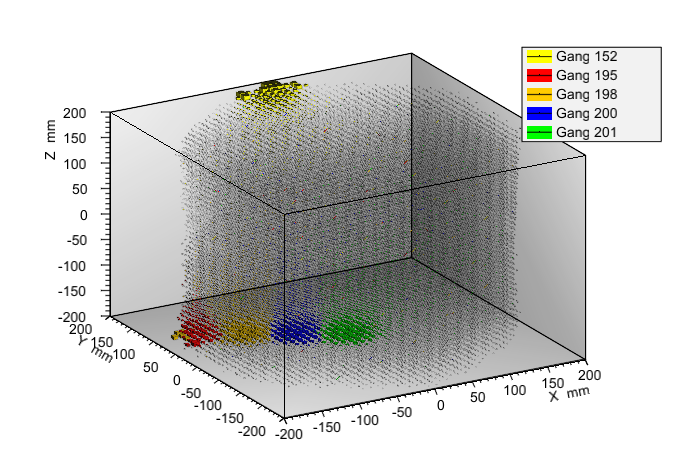
\includegraphics[keepaspectratio=true,width=\textwidth]{Lightmap_viz.png}
\end{center}
\renewcommand{\baselinestretch}{1}
\small\normalsize
\begin{quote}
\caption{Lightmap position-dependence $R(\vec{x})$ for selected APD gangs.}
\label{fig:Lightmap3DPlot_unzoomed}
\end{quote}
\end{figure}
\renewcommand{\baselinestretch}{2}
\small\normalsize

\begin{figure}
\begin{center}
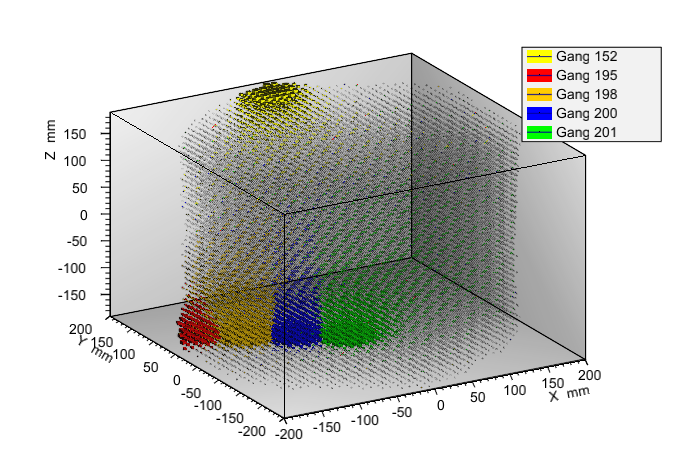
\includegraphics[keepaspectratio=true,width=\textwidth]{Lightmap_viz_zoom.png}
\end{center}
\renewcommand{\baselinestretch}{1}
\small\normalsize
\begin{quote}
\caption{Lightmap position-dependence $R(\vec{x})$ for selected APD gangs.  Here extreme anode positions are omitted to permit better contrast for the lightmap in the fiducial volume.}
\label{fig:Lightmap3DPlot_zoomed}
\end{quote}
\end{figure}
\renewcommand{\baselinestretch}{2}
\small\normalsize

\begin{figure}
\begin{center}
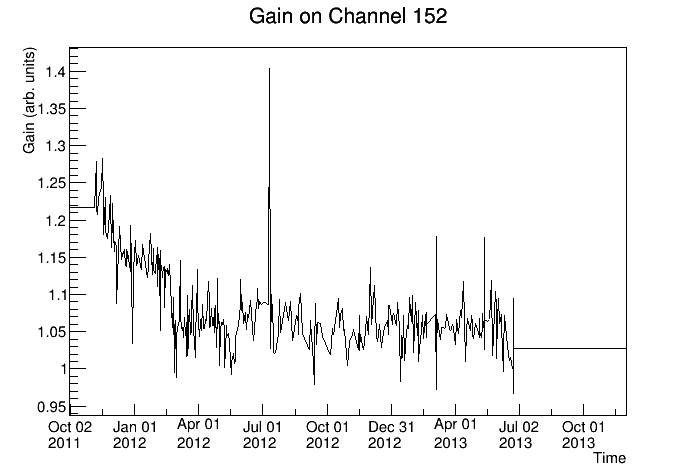
\includegraphics[keepaspectratio=true,width=\textwidth]{gainfunc_152.png}
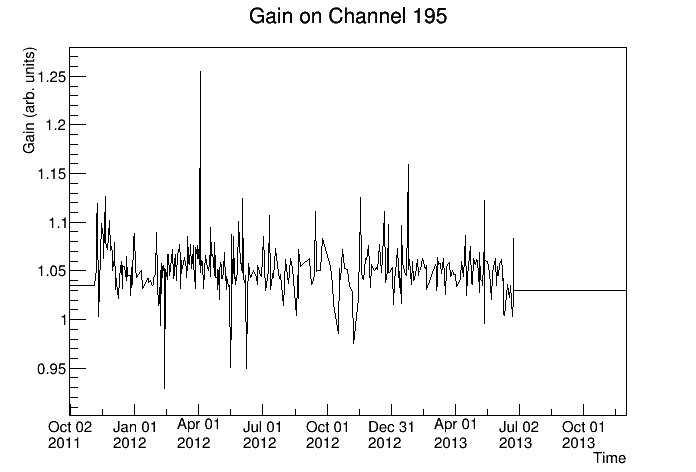
\includegraphics[keepaspectratio=true,width=\textwidth]{gainfunc_195.png}
\end{center}
\renewcommand{\baselinestretch}{1}
\small\normalsize
\begin{quote}
\caption{Functions $S(t)$ for selected channels.}
\label{fig:LightmapGainFunc1}
\end{quote}
\end{figure}
\renewcommand{\baselinestretch}{2}
\small\normalsize

\begin{figure}
\begin{center}
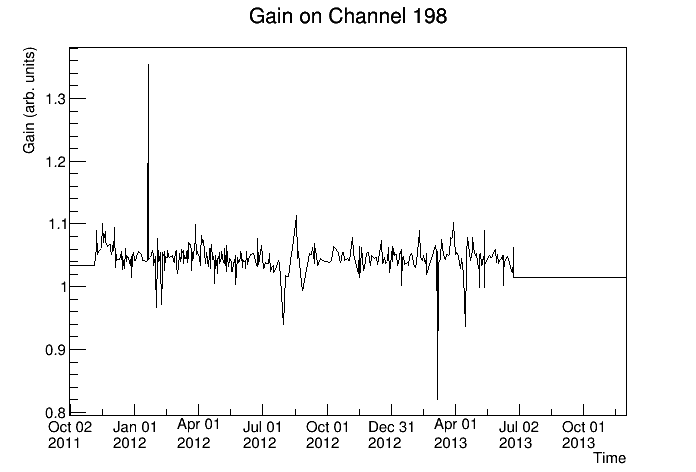
\includegraphics[keepaspectratio=true,width=\textwidth]{gainfunc_198.png}
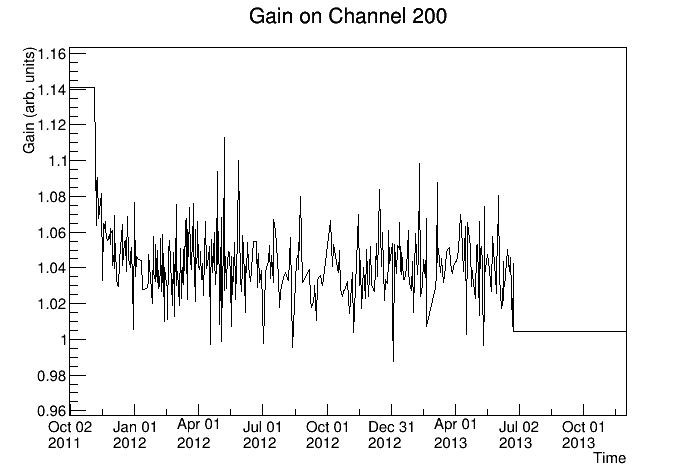
\includegraphics[keepaspectratio=true,width=\textwidth]{gainfunc_200.png}
\end{center}
\renewcommand{\baselinestretch}{1}
\small\normalsize
\begin{quote}
\caption{Functions $S(t)$ for selected channels.}
\label{fig:LightmapGainFunc2}
\end{quote}
\end{figure}
\renewcommand{\baselinestretch}{2}
\small\normalsize

\begin{figure}
\begin{center}
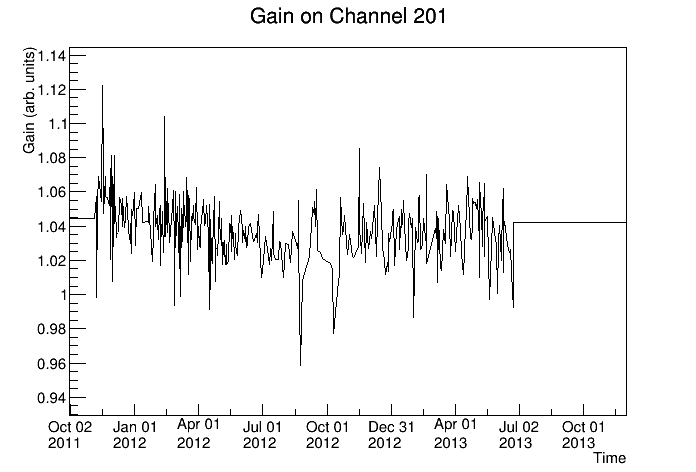
\includegraphics[keepaspectratio=true,width=\textwidth]{gainfunc_201.png}
\end{center}
\renewcommand{\baselinestretch}{1}
\small\normalsize
\begin{quote}
\caption{Functions $S(t)$ for selected channels.}
\label{fig:LightmapGainFunc3}
\end{quote}
\end{figure}
\renewcommand{\baselinestretch}{2}
\small\normalsize

Although it is not strictly necessary to be able to visually inspect the lightmap for it to be useful, nevertheless it is reassuring to see that the lightmap is qualitatively similar to intuitive expectations of how light should propagate through the detector.  We have chosen to store the position-dependent $R(\vec{x})$ for each APD gang as a set of ROOT TH3D objects, and fortunately ROOT provides a number of excellent plotting features suitable for a three-dimensional dataset.  In figure~\ref{fig:Lightmap3DPlot_unzoomed}, it is possible to view the values of $R(\vec{x})$ for a sample of gangs on top of each other.  Larger boxes and denser color indicates a higher yield on the APD gang in question, and it is immediately apparent that events near the anodes produce light which is highly concentrated on a single APD gang.

Figure~\ref{fig:Lightmap3DPlot_unzoomed} shows the highest yield on the very boundary of the detector, well outside of our fiducial volume; to permit us to more easily view contrast inside of the detector, figure~\ref{fig:Lightmap3DPlot_zoomed} shows the same map while omitting the most extreme bin near either anode.  Viewing this map, we can see more interesting characteristics of the lightmap:
\begin{itemize}
\item Events near the anodes show a high pulse concentration on the one gang nearest to their position; however, even deep into the detector near the cathode it is still possible to see the higher concentration of pulse magnitude on the gang directly aligned with the event.
\item We can also see, from gang 201 (green) in this visualization, that events can produce significant pulse magnitudes on APD gangs which which they are not directly aligned (in the Z direction); yield on gang 201 can be seen to decrease smoothly in all directions.
\item APD gangs in the corners of the detector, such as gang 195 (red), are not effective at measuring light from events which are far away; even directly above gang 195, it is clear that gang 198 is more effective at collecting light farther away than about five to ten centimeters.  This can be attributed to the reflection of photons by teflon, which may enhance the light yield on gangs which are not hidden in corners.
\end{itemize}

Figures~\ref{fig:LightmapGainFunc1}, \ref{fig:LightmapGainFunc2}, and~\ref{fig:LightmapGainFunc3} show the functions $S(t)$ for the same sample of gangs.  The vertical scale can be treated as having arbitrary units; we note that all of these functions lie roughly around $1$, which is attributed to the initial placement of $S(t) = 1$ in algorithm~\ref{alg:LightmapScheme}.  We draw the following primary observations from these plots:
\begin{itemize}
\item Many of the gangs show their values of $S(t)$ decreasing rapidly up to around February 2012; some of the gangs also show a sharp decrease in value at that point.  The decrease in gain corresponds with observations which were made at the time, leading to a decision to replace electronics on some APD channels on February 23, 2012.  Thus, we do see ``real" features from these plots.
\item The functions $S(t)$ are otherwise dominated by jitter between points, indicating that we do not collect enough statistics from each run to sufficiently constrain $S(t)$.  This is taken as the strongest evidence that we should use a coarser time binning for $S(t)$, as described in section~\ref{sec:LightmapFunctionParametrization}.  Preliminary work has been performed to do this with more recent lightmaps, but no studies have evaluated the impact on energy resolution.
\item Individual points on these functions may spike by as much as $40\%$.  These points have been investigated, and their cause is not understood.  These jumps, along with the overall jitter, will certainly be reduced by the use of a coarser time binning.
\end{itemize}

\section{Summary}

In this chapter we have described the generation of an individual-APD lightmap which characterizes the expected pulse magnitude on each APD channel as a function of scintillation origin, calendar time, and the quantity of energy.  The two key steps to this process are the use of the full dataset for extra statistics and the assumption that the lightmap is separable between position and time coordinates, as shown in equation~\ref{eqn:SeparableLightmap}.  Previous lightmaps could only characterize the light yield on large sums of waveforms; by providing a full lightmap for every channel, we enable the denoising algorithm of chapter~\ref{ch:DenoisingTheory} to make use of channel-by-channel pulse and noise information, so this lightmap is a key component of denoising and the improvement in resolution presented in section~\ref{sec:ResultComparison}.


\renewcommand{\thechapter}{4}
\chapter{Denoising Theory}

As has been discussed, the performance of double-beta experiments like EXO-200 is partially determined by their energy resolution.  In EXO-200, the energy resolution is limited by the scintillation energy resolution, which in turn is dominated by electronic noise in the APDs.  Significant effort must therefore be expended to understand and reduce the noise in the scintillation signals.

\begin{figure}
\begin{center}
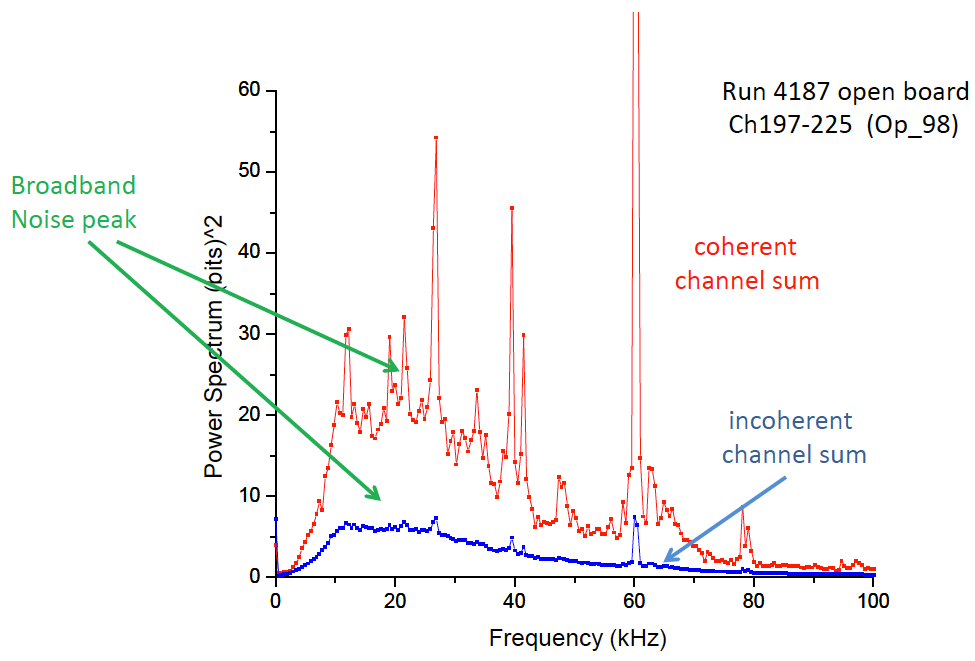
\includegraphics[keepaspectratio=true,width=\textwidth]{APDNoisePowerSpectrum.png}
\end{center}
\renewcommand{\baselinestretch}{1}
\small\normalsize
\begin{quote}
\caption{Coherent and incoherent noise power spectra for a sample set of APD channels without signal shaping.~\cite{ElectronicsUpgradeReport}}
\label{fig:APDNoisePowerSpectrum}
\end{quote}
\end{figure}
\renewcommand{\baselinestretch}{2}
\small\normalsize

When the noise in the APDs is studied, it was found that the individual APD channels met targetted root-mean-square noise levels of 2000 electrons.  However, rather than observing the noise on summed APD channels increase proportionally to the square root of the number of channels, the summed APD noise is roughly two to three times higher than projected.  This worse-than-expected scaling of the noise with channels indicates that noise across different channels is correlated, and further analysis confirms that the bulk of the noise on an unshaped APD waveform is correlated with other channels, as shown in Figure~\ref{fig:APDNoisePowerSpectrum}.  There are many possible sources of coherent noise in the hardware, and reducing the amount of coherent noise is a topic for further research.~\cite{ElectronicsUpgradeReport}

However, the observation that coherent noise is the dominant source of noise in the APDs, and thus also the limiting factor in EXO-200's energy resolution, means that it should be possible to exploit these correlations and reduce the level of noise in offline analysis.  This chapter will describe a scheme to accomplish that goal and produce an optimal estimate of scintillation energy which takes noise correlations into account.

It is worth noting that in fact there are a number of different qualitative approaches to reducing the noise levels in the scintillation channel.  In casual terms, we will refer to "passive" approaches as those in which components of our signals are weighted more or less heavily based on their relative signal-to-noise content.  "Active" approaches, by contrast, will be classified as those which attempt to improve the signal-to-noise content of signal components.  We have identified the following three types of denoising:
\begin{description}
\item[Frequency weighting] \hfill \\
On a given channel signal, weight more heavily the frequency components which contain larger signal-to-noise ratio.  This passive denoising scheme requires knowledge of the shapes in fourier space of a signal and the power spectrum of the noise.

\item[Channel weighting] \hfill \\
Different channels may have different levels of noise, so some may generally have higher-quality signals.  More importantly, though, the amount of signal on a given channel depends strongly on the proximity of the APD gang to the source of scintillation within the detector.  This passive denoising scheme therefore allows us to weight more heavily the channels which have more scintillation, provided we can identify these weights on an event-by-event basis.  This requires knowledge of the magnitude of noise on each channel and of the correspondence between event position and signal magnitude on each APD gang; the latter is described by the lightmap, described earlier.

\item[Noise subtraction] \hfill \\
This active form of denoising consists of using correlations between noise on different channels to produce a better estimate of the noise component of signals than each signal taken independently could provide.  To accomplish this, we will require detailed information about the pairwise noise correlations across channels at each frequency.
\end{description}

In the following, we will describe a general linear operator on the APD signals which in principle can accomplish each of these forms of denoising, and we will presume that all of the described inputs are available; by identifying the parameters for that linear operator which are optimal, we can be confident that the denoising operator we produce will accomplish all three forms of denoising described above.

\section{Setup}

We first establish a number of notational conventions:
\begin{itemize}
\item $i$, $j$ will represent indices over APD channels.
\item $a$, $b$, $c$ will represent indices of signals in an event.
\item $\tau$ will represent the time indices of a discrete waveform; $t_a$ represents the calendar time of a signal $a$.
\item $f$, $g$ will represent the frequency indices of Fourier-transformed waveforms.
\item For a waveform $*[\tau]$, we will represent the discrete Fourier transform of that waveform with $\widetilde{*}[f]$, where the particular convention used to evaluate the Fourier transform is not significant.
\item For a Fourier-transformed waveform $\widetilde{*}[f]$, we denote the real and imaginary parts of that waveform by $\widetilde{*}^R[f]$ and $\widetilde{*}^I[f]$, respectively.
\item For an unknown parameter $*$, the symbol $\widehat{*}$ will identify an estimator for $*$.
\item For an expression $*$ containing random variables, $\left<*\right>$ is the expectation value of $*$.
\end{itemize}

We describe the data as a collection of discretely sampled waveforms, $X_i[\tau]$.  We assume that all signal times and shapes are already known, so we can model the waveforms by $X_i[\tau] = \sum_a M_{ia}Y_{ia}[\tau] + N_i[\tau] + b_i$, where $Y$ is the shape of signal $a$ on channel $i$, $M$ is the magnitude of that signal, and $N$ and $b$ represent the electronic noise and baseline, respectively, of the channel.

To break the degeneracy between $M$ and $Y$, we choose to fix the magnitude of the template signal $Y$.  We choose to require that the signal $Y$ has a magnitude of one, as described in figure~\ref{fig:SampleAPDTemplates}.  This implies that for a typical single-site $2615$-keV deposit, the average values of $M_i$ should be equal to the values of the lightmap $L_i(\vec{x},t)$ described earlier.

Noise correlations will be much simpler in frequency space, so we take the Fourier transform and drop the zero-frequency component to obtain \[\widetilde{X}_i[f] = \sum_a M_{ia}\widetilde{Y}_{ia}[f] + \widetilde{N}_i[f].\]

\section{The Signal Model}

It is first important to characterize the response of the APDs to energy deposits in EXO-200.  This will require us to understand the signal amplification of the detector at each physical stage, as well as the noise introduced by each of these processes.  We will describe both in detail here.

\subsection{APD Noise}

We will assume that there are two sources of noise in this model.  First, the electronic noise $N_i[\tau]$ is assumed to be random.  We require that noise with different frequencies is uncorrelated:
\[\left< \widetilde{N}_i[f] \widetilde{N}_j[g] \right> = 0 \text{~when~} f \ne g.\]
The noise correlations $\left< \widetilde{N}_i[f] \widetilde{N}_j[f] \right>$ are assumed to be known; our means for measuring them are described [ELSEWHERE].

The second random variable will be the magnitude of the signal itself, $M_{ia}$.  When an energetic decay occurs in bulk of the detector, it will release some number of photons.  We will denote the number of photons released by signal $a$ by $P^{(0)}_a$, and this is the parameter we wish to measure.  However, the magnitude signal actually observed on APD channels number of photons actually collected by sensors is a random variable whose distribution depends on $P^{(0)}_a$, and we will now identify the chain of events which produce it.

First, each APD gang $i$ has some number $P^{(1)}_{ia}$ of photons which reach them.  The mean fraction of photons reaching a particular gang $i$ from position $\vec{x}_a$, $f_i(\vec{x}_a)$, is assumed to be known; however, the initial paths of the optical photons emitted from the source, their trajectories through the Xenon, and their success in reflecting off of teflon are all random, so we treat $P^{(1)}_{ia}$ as a Poisson-distributed random variable with mean $f_i(\vec{x}_a)P^{(0)}_a$.  A typical deposit from a $\beta\beta 0\nu$ event may deposit $10-100$ photons on each APD gang [CHECK THIS NUMBER], depending strongly on the location of the deposit; thus, we find that the Poisson noise on a single APD channel may be quite significant.

Additionally, the number of photons reaching different gangs are not uncorrelated; since a photon which reaches gang $i$ cannot deposit on a different gang $j$, $P^{(1)}_{ia}$ and $P^{(1)}_{ja}$ are anticorrelated for different gangs $i \ne j$.  This process is described by a multinomial distribution.  Explicitly, we can identify the expectation values of a multinomial distribution:
\begin{itemize}
\item $\left< P^{(1)}_{ia} \right> = f_i(\vec{x}_a)P^{(0)}_a$
\item $\left< P^{(1)}_{ia} P^{(1)}_{jb} \right> = \left< P^{(1)}_{ia} \right> \left< P^{(1)}_{jb} \right> + \left[ f_i(\vec{x}_a)\delta_{ij} - f_i(\vec{x}_a)f_j(\vec{x}_a) \right] P^{(0)}_a \delta_{ab}$
\end{itemize}

Following the random process associated with photons reaching the APD gangs, there is also randomness associated with signal amplification internally in the APDs.  These processes are described in detail in~\cite{EXOLAAPD}, but we can summarize that:

\begin{enumerate}
\item Optical photons in the liquid xenon arrive at the active layer of the APDs have a wavelength of roughly $178$ nm, meaning that each optical photon has an energy of roughly $7.0$ eV.  The energy required to produce one electron-hole pair in silicon is roughly $3.66$ eV, which means that each incident photon produces roughly $1.9$ electron-hole pairs; we will define $P^{(2)}_{ia}$ to be the number of electron-hole pairs actually produced from $P^{(1)}_{ia}$ incident photons.  The corresponding Fano factor for electrons produced in silicon is roughly $0.1$, meaning that in addition to the uncertainty in $P^{(1)}_{ia}$ which we have already characterized, there is an additional uncorrelated variance in $P^{(2)}_{ia}$ equal to $0.1 \left<P^{(2)}_{ia}\right>$.  The correlations in the parameters $P^{(2)}_{ia}$ are therefore:
\[\left< P^{(2)}_{ia} \right> = 1.9 \cdot P^{(1)}_{ia}\]
\[\left< P^{(2)}_{ia} P^{(2)}_{jb} \right> = (1.9)^2\left< P^{(1)}_{ia} P^{(1)}_{jb} \right> + 0.1 \left< P^{(2)}_{ia}\right> \delta_{ij}\delta_{ab}\]
\item Electron-hole pairs are then amplified by an avalanche process inside the APDs.  The magnitude of this gain is APD-dependent, generally on the order of $200-300$, and can be identified by a time-dependent quantity $G^P_i(t)$; we will call the number of output electrons $P^{(3)}_{ia}$.  In addition to amplification of existing noise in $P^{(2)}_{ia}$, two additional source of noise are introduced.  First, there is statistical variance in the amplification experienced by each electron due to the randomness of the avalanche process.  This variance is dependent on many factors, including the gain, and scales like the square root of the number of electrons; we define the variance on the gain experienced by a single electron as $\sigma^2_{G_i}(t)$.  Second, there are gain non-uniformities in the diode volume, which contribute variance proportional to the square of the number of initial electron-hole pairs; we will identify the proportionality constant as $\sigma^2_{NU}$, which may depend on time and APD gang.  The magnitude of this uncertainty is not well-known, but may be significant.  The correlations in the parameters $P^{(3)}_{ia}$ are therefore:
\[\left< P^{(3)}_{ia} \right> = G^P_i(t_a)P^{(2)}_{ia}\]
\[\left< P^{(3)}_{ia} P^{(3)}_{jb} \right> = G^P_i(t_a)G^P_j(t_b) \left< P^{(2)}_{ia} P^{(2)}_{jb} \right> + \left[P^{(2)}_{ia}\sigma^2_{G_i}(t_a) + \left(P^{(2)}_{ia}\right)^2\sigma^2_{NU}\right]\delta_{ij}\delta_{ab}\]
\end{enumerate}

Finally, there is amplification $G^{E}_i(t)$ associated with the electronics of the APDs which is dependent on time and channel.  This includes preamplifier gain, shaper gain, gain associated with the shaping times, and conversion from voltage to ADC counts.  We assume that no signal-dependent noise is introduced during this stage, but there is constant electronic noise $N_i[\tau]$ which has been described above.  Additionally, the APDs can contribute noise in the form of a dark current which is uncorrelated with signals; this is inseparable from the electronic noise, and so we absorb it into our description of $N_i[\tau]$.

\subsection{APD Signals and Noise}

We have already characterized the overall gain of the APDs using the lightmap described earlier.  We know that a typical single-site deposit of $2615$ keV at position $\vec{x}$ and time $t$ will produce a signal with expected magnitude $L_i(\vec{x},t)$ on APD channel $i$.  We must now connect this empirical understanding of our APD signals with the physical understanding in terms of photons and electrons described above.

We have identified the number of photons created by an event $a$ as $P^{(0)}_a$.  In reality, an ideal scintillation measurement can only measure this quantity, and not the true energy of the event -- there is randomness in the number of photons produced by a known-energy deposit, so $P^{(0)}_a$ will not be perfectly correlated with the energy $E_a$ of the event.  However, the number of photons generated is a difficult parameter to understand empirically, and all of our calibrations occur at a known energy even though the corresponding number of deposited photons is unknown.

Simulations using NEST~\cite{NESTpaper} which have been performed within the EXO group by Liangjian Wen at our bulk electric field indicate that we can expect roughly $82,000$ photons from a $2615$-keV gamma deposit.  We will identify this parameter with $c$, and express the average relation between energy and photon yield in EXO-200 by
$P^{(0)} = c \cdot E$,
where $E$ is the energy measured in units of $2615$ keV.  We will treat this relationship as exact, and attempt to measure $E$ rather than $P^{(0)}$; this means that when we speak of measuring the energy of an event using the APD signals, we really are referring to measuring the "scintillation energy," or a parameter proportional to the number of emitted photons which on average will equal the true energy of the deposit.

Ignoring variances for a moment, we can combine all of the expectation values for numbers of photons or ADC counts above to state that on average,
\[M_{ia} = 1.9 \cdot c f_i(\vec{x}_a) G^P_i(t_a) G^E_i(t_a) E_a.\]
We can compare this to our empirical lightmap measurements, which are expressed by $M_{ia} = L_i(\vec{x}_a,t_a) E_a$,
and we conclude that:
\[ L_i(\vec{x},t) = 1.9 \cdot c f_i(\vec{x}) G^P_i(t) G^E_i(t).\]

We recall that it is assumed the lightmap is a separable function, $L_i(\vec{x},t) = R_i(\vec{x})S_i(t)$, and we can provide the two proportionalities:
\[ R_i(\vec{x}) \propto f_i(\vec{x}) \]
\[ S_i(t) \propto G^P_i(t) G^E_i(t).\]

Although $G^E_i(t)$ is in principle time-dependent, due to environmental effects on the APD electronics and occasional replacement of electronics cards for certain channels, precision data on its value is not readily available.  Instead, we use a time-independent estimate $G^E_i(t) = 1.1 \cdot 10^{-3}$ ADC counts per electron emitted from the APD; the uncertainty in this figure is dominated by uncertainty in the preamplifier gains, which are controlled by a roughly $5$ pF capacitor.  Other contributors to the gain include shaper gain of $21.2$ (from a combination of amplification and shaping) and a full-scale digitizer range of $2.5$ volts for $12$-bit digitization.

We do have independent measurements of the APD gains $G^P_i(t)$ available from laser calibration runs.  These special runs allow a laser to shine into the detector from a fixed point and with a stable amplitude while the bias voltages on the APDs are varied from an effective unity gain to our standard voltage settings.  Using these measurements, we are able to measure $G^P_i(t)$ at weekly intervals from September 2012 to the present time.  Before September 2012, some less-reliable laser data is available, but results from that data are not readily available as of this writing.

It would be possible, and should be a goal for future improvements, to make use of this full range of laser data.  However, the laser data provides a less uniform history of APD gains over the full data-taking window of EXO-200 from September 2011 to November 2013, and it is much easier to track time-dependent behavior from Thorium source data which have been collected regularly throughout that period.  As a result, a compromise is used to characterize $G^P_i(t)$.  One particular laser run, run 4540 (taken on December 13, 2012), is used to fix $G^P_i(t_{4540})$, and the function is extrapolated using Thorium source data with:
\[G^P_i(t) \approx G^P_i(t_{4540}) \cdot S_i(t)/S_i(t_{4540}).\]
This assumption makes use of the approximation that $G^E_i(t)$ is roughly constant in time, which is probably only accurate to one significant figure; therefore when an electronics change is made to a channel, we can expect that the accuracy of $G^P_i(t)$ is no better than one significant figure.  These results mean that we can also estimate with the same level of accuracy:
\[f_i(\vec{x}) \approx \frac{S_i(t_{4540})}{G^P_i(t_{4540})} \cdot \frac{R_i(\vec{x})}{1.9 \cdot c G^E_i(t)}.\]

It is then possible to express the full correlations in signal magnitudes in terms of the scintillation energies of deposits as:
\begin{align*}
\left< M_{ia} \right> &= L_i(\vec{x}_a,t_a) E_a \\
\begin{split}
\left< M_{ia} M_{jb} \right> &= L_i(\vec{x}_a,t_a)L_j(\vec{x}_b,t_b) E_a E_b \left[1 + \frac{\sigma^2_{NU}}{\left(G^P_i(t)\right)^2} \delta_{ij}\delta_{ab} \right] \\
&\quad - L_i(\vec{x}_a,t_a) L_j(\vec{x}_a,t_a) E_a \delta_{ab}/c \\
&\quad + L_i(\vec{x}_a,t_a) G^E_i(t) E_a \delta_{ij} \delta_{ab} \left[\left(0.1 + 1.9\right)G^P_i(t) + \frac{\sigma^2_{G_i}(t)}{G^P_i(t)}\right].
\end{split}\end{align*}
\begin{comment}
THE FOLLOWING IS MY WORK IN EXPANDING THE M_M CORRELATIONS.
IF NEEDED, IT CAN BE UNCOMMENTED AND IS VALID LATEX CODE.

\[ \left< M_{ia} M_{jb} \right> = G^E_i(t) G^E_j(t) \left<P^{(3)}_{ia}P^{(3)}_{jb} \right> \]

\[ \left< M_{ia} M_{jb} \right> = G^E_i(t) G^E_j(t) \left( G^P_i(t)G^P_j(t) \left< P^{(2)}_{ia} P^{(2)}_{jb} \right> + \left[P^{(2)}_{ia}\sigma^2_{G_i}(t) + \left(P^{(2)}_{ia}\right)^2\sigma^2_{NU}\right]\delta_{ij}\delta_{ab}\right)\]

\begin{equation*}\begin{split}
\left< M_{ia} M_{jb} \right> ={}& G^E_i(t) G^E_j(t) G^P_i(t)G^P_j(t) \left< P^{(2)}_{ia} P^{(2)}_{jb} \right> \\
 & + G^E_i(t) G^E_j(t) \left[P^{(2)}_{ia}\sigma^2_{G_i}(t) + \left(P^{(2)}_{ia}\right)^2\sigma^2_{NU}\right]\delta_{ij}\delta_{ab}
\end{split}\end{equation*}

\begin{equation*}\begin{split}
\left< M_{ia} M_{jb} \right> ={}& G^E_i(t) G^E_j(t) G^P_i(t)G^P_j(t) \left( (1.9)^2\left< P^{(1)}_{ia} P^{(1)}_{jb} \right> + 0.1 \left< P^{(2)}_{ia}\right> \delta_{ij}\delta_{ab} \right) \\
 & + G^E_i(t) G^E_j(t) \left[1.9 \cdot P^{(1)}_{ia}\sigma^2_{G_i}(t) + (1.9)^2 \left(P^{(1)}_{ia}\right)^2\sigma^2_{NU}\right]\delta_{ij}\delta_{ab}
\end{split}\end{equation*}

\begin{equation*}\begin{split}
\left< M_{ia} M_{jb} \right> ={}& (1.9)^2 G^E_i(t) G^E_j(t) G^P_i(t)G^P_j(t) \left< P^{(1)}_{ia} P^{(1)}_{jb} \right> \\
& + 0.1 \cdot 1.9 \cdot G^E_i(t) G^E_j(t) G^P_i(t)G^P_j(t) P^{(1)}_{ia} \delta_{ij}\delta_{ab} \\
 & + G^E_i(t) G^E_j(t) \left[1.9 \cdot P^{(1)}_{ia}\sigma^2_{G_i}(t) + (1.9)^2 \left(P^{(1)}_{ia}\right)^2\sigma^2_{NU}\right]\delta_{ij}\delta_{ab}
\end{split}\end{equation*}

\begin{equation*}\begin{split}
\left< M_{ia} M_{jb} \right> ={}& (1.9)^2 G^E_i(t) G^E_j(t) G^P_i(t)G^P_j(t) \left< P^{(1)}_{ia} P^{(1)}_{jb} \right> \\
 & + G^E_i(t) G^E_j(t) \left[1.9 \cdot P^{(1)}_{ia}\sigma^2_{G_i}(t) + (1.9)^2 \left(P^{(1)}_{ia}\right)^2\sigma^2_{NU} + 0.1 \cdot 1.9 \cdot G^P_i(t)G^P_j(t) P^{(1)}_{ia}\right]\delta_{ij}\delta_{ab}
\end{split}\end{equation*}

\begin{equation*}\begin{split}
\left< M_{ia} M_{jb} \right> ={}& (1.9)^2 G^E_i(t) G^E_j(t) G^P_i(t)G^P_j(t) \left< P^{(1)}_{ia} P^{(1)}_{jb} \right> \\
 & + 1.9\left[\sigma^2_{G_i}(t) + 1.9 \cdot P^{(1)}_{ia} \sigma^2_{NU} + 0.1 \cdot G^P_i(t)G^P_j(t) \right] \left(G^E_i(t)\right)^2 P^{(1)}_{ia} \delta_{ij}\delta_{ab}
\end{split}\end{equation*}

\begin{equation*}\begin{split}
\left< M_{ia} M_{jb} \right> ={}& (1.9)^2 G^E_i(t) G^E_j(t) G^P_i(t)G^P_j(t) \left< P^{(1)}_{ia} \right> \left< P^{(1)}_{jb} \right> \\
& + (1.9)^2 G^E_i(t) G^E_j(t) G^P_i(t)G^P_j(t)\left[ f_i(x,y,z)\delta_{ij} - f_i(x,y,z)f_j(x,y,z) \right] P^{(0)}_a \delta_{ab}  \\
 & + 1.9\left[\sigma^2_{G_i}(t) + 1.9 \cdot P^{(1)}_{ia} \sigma^2_{NU} + 0.1 \cdot G^P_i(t)G^P_j(t) \right] \left(G^E_i(t)\right)^2 P^{(1)}_{ia} \delta_{ij}\delta_{ab}
\end{split}\end{equation*}

\begin{equation*}\begin{split}
\left< M_{ia} M_{jb} \right> ={}& (1.9)^2 G^E_i(t) G^E_j(t) G^P_i(t)G^P_j(t) f_i(x,y,z) f_j(x,y,z) \left(P^{(0)}_a\right)^2 \\
& + (1.9)^2 G^E_i(t) G^E_j(t) G^P_i(t)G^P_j(t)\left[ f_i(x,y,z)\delta_{ij} - f_i(x,y,z)f_j(x,y,z) \right] P^{(0)}_a \delta_{ab}  \\
 & + 1.9\left[\sigma^2_{G_i}(t) + 1.9 \cdot f_i(x,y,z) P^{(0)}_a \sigma^2_{NU} + 0.1 \cdot G^P_i(t)G^P_j(t) \right] \left(G^E_i(t)\right)^2 f_i(x,y,z) P^{(0)}_a \delta_{ij}\delta_{ab}
\end{split}\end{equation*}

\begin{equation*}\begin{split}
\left< M_{ia} M_{jb} \right> ={}& (1.9)^2 G^E_i(t) G^E_j(t) G^P_i(t)G^P_j(t) f_i(x,y,z) f_j(x,y,z) c^2 E^2_a \\
& + (1.9)^2 G^E_i(t) G^E_j(t) G^P_i(t)G^P_j(t)\left[ f_i(x,y,z)\delta_{ij} - f_i(x,y,z)f_j(x,y,z) \right] c E_a \delta_{ab}  \\
 & + 1.9\left[\sigma^2_{G_i}(t) + 1.9 \cdot f_i(x,y,z) c E_a \sigma^2_{NU} + 0.1 \cdot G^P_i(t)G^P_j(t) \right] \left(G^E_i(t)\right)^2 f_i(x,y,z) c E_a \delta_{ij}\delta_{ab}
\end{split}\end{equation*}

\begin{equation*}\begin{split}
\left< M_{ia} M_{jb} \right> ={}& L_i(x,y,z,t)L_j(x,y,z,t) E^2_a \\
& + (1.9)^2 G^E_i(t) G^E_j(t) G^P_i(t)G^P_j(t) f_i(x,y,z)\delta_{ij} c E_a \delta_{ab}  \\
& - (1.9)^2 G^E_i(t) G^E_j(t) G^P_i(t)G^P_j(t) f_i(x,y,z)f_j(x,y,z) c E_a \delta_{ab} \\
 & + 1.9\left[\sigma^2_{G_i}(t) + 1.9 \cdot f_i(x,y,z) c E_a \sigma^2_{NU} + 0.1 \cdot G^P_i(t)G^P_j(t) \right] \left(G^E_i(t)\right)^2 f_i(x,y,z) c E_a \delta_{ij}\delta_{ab}
\end{split}\end{equation*}

\begin{equation*}\begin{split}
\left< M_{ia} M_{jb} \right> ={}& L_i(x,y,z,t)L_j(x,y,z,t) E^2_a \\
& + L_i(x,y,z,t) (1.9)  G^E_i(t) G^P_i(t) \delta_{ij}  E_a \delta_{ab}  \\
& - L_i(x,y,z,t)     (1.9) G^E_j(t) G^P_j(t) f_j(x,y,z) E_a \delta_{ab} \\
 & + 1.9\left[\sigma^2_{G_i}(t) + 1.9 \cdot f_i(x,y,z) c E_a \sigma^2_{NU} + 0.1 \cdot \left(G^P_i(t)\right)^2 \right] \left(G^E_i(t)\right)^2 f_i(x,y,z) c E_a \delta_{ij}\delta_{ab}
\end{split}\end{equation*}

\begin{equation*}\begin{split}
\left< M_{ia} M_{jb} \right> ={}& L_i(x,y,z,t)L_j(x,y,z,t) E^2_a \\
& + L_i(x,y,z,t) (1.9)  G^E_i(t) G^P_i(t) E_a \delta_{ij} \delta_{ab}  \\
& - L_i(x,y,z,t) L_j(x,y,z,t) E_a \delta_{ab}/c \\
& + (1.9)\sigma^2_{G_i}(t)\left(G^E_i(t)\right)^2 f_i(x,y,z) c E_a \delta_{ij}\delta_{ab} \\
& + (1.9)^2 f_i(x,y,z) c E_a \sigma^2_{NU} \left(G^E_i(t)\right)^2 f_i(x,y,z) c E_a \delta_{ij}\delta_{ab} \\
& + (1.9) (0.1) \left(G^P_i(t)\right)^2 \left(G^E_i(t)\right)^2 f_i(x,y,z) c E_a \delta_{ij}\delta_{ab}
\end{split}\end{equation*}

\begin{equation*}\begin{split}
\left< M_{ia} M_{jb} \right> ={}& L_i(x,y,z,t)L_j(x,y,z,t) E^2_a \\
& + (1.9)^2 f^2_i(x,y,z) \sigma^2_{NU} \left(G^E_i(t)\right)^2 c^2 E^2_a \delta_{ij}\delta_{ab} \\
& - L_i(x,y,z,t) L_j(x,y,z,t) E_a \delta_{ab}/c \\
& + L_i(x,y,z,t) (1.9)  G^E_i(t) G^P_i(t) E_a \delta_{ij} \delta_{ab}  \\
& + (1.9)\sigma^2_{G_i}(t)\left(G^E_i(t)\right)^2 f_i(x,y,z) c E_a \delta_{ij}\delta_{ab} \\
& + L_i(x,y,z,t) (0.1) G^P_i(t) G^E_i(t) E_a \delta_{ij}\delta_{ab}
\end{split}\end{equation*}

\begin{equation*}\begin{split}
\left< M_{ia} M_{jb} \right> ={}& L_i(x,y,z,t)L_j(x,y,z,t) E^2_a \\
& + L^2_i(x,y,z,t) \sigma^2_{NU} E^2_a \delta_{ij}\delta_{ab}/\left(G^P_i(t)\right)^2 \\
& - L_i(x,y,z,t) L_j(x,y,z,t) E_a \delta_{ab}/c \\
& + L_i(x,y,z,t) (1.9)  G^E_i(t) G^P_i(t) E_a \delta_{ij} \delta_{ab}  \\
& + L_i(x,y,z,t) \sigma^2_{G_i}(t)G^E_i(t) E_a \delta_{ij}\delta_{ab}/G^P_i(t) \\
& + L_i(x,y,z,t) (0.1) G^P_i(t) G^E_i(t) E_a \delta_{ij}\delta_{ab}
\end{split}\end{equation*}

\begin{equation*}\begin{split}
\left< M_{ia} M_{jb} \right> ={}& L_i(x,y,z,t)L_j(x,y,z,t) E^2_a \left[1 + \frac{\sigma^2_{NU}}{\left(G^P_i(t)\right)^2} \delta_{ij}\delta_{ab} \right] \\
& - L_i(x,y,z,t) L_j(x,y,z,t) E_a \delta_{ab}/c \\
& + L_i(x,y,z,t) \sigma^2_{G_i}(t)G^E_i(t) E_a \delta_{ij}\delta_{ab}/G^P_i(t) \\
& + L_i(x,y,z,t) (1.9 + 0.1)  G^E_i(t) G^P_i(t) E_a \delta_{ij} \delta_{ab}
\end{split}\end{equation*}

\begin{equation*}\begin{split}
\left< M_{ia} M_{jb} \right> ={}& L_i(x,y,z,t)L_j(x,y,z,t) E^2_a \left[1 + \frac{\sigma^2_{NU}}{\left(G^P_i(t)\right)^2} \delta_{ij}\delta_{ab} \right] \\
& - L_i(x,y,z,t) L_j(x,y,z,t) E_a \delta_{ab}/c \\
& + L_i(x,y,z,t) G^E_i(t) E_a \delta_{ij} \delta_{ab} \left[\left(0.1 + 1.9\right)G^P_i(t) + \frac{\sigma^2_{G_i}(t)}{G^P_i(t)}\right]
\end{split}\end{equation*}
\end{comment}

We combine this with our knowledge of the noise coefficients:
\begin{align*}
\left< \widetilde{N}_i[f] \right> &= 0 \\
\left< \widetilde{N}_i[f] \widetilde{N}_j[g] \right> &= \left\{ \begin{aligned}
0~ &\text{if}~ f \ne g \\
\text{known}~ &\text{if}~ f = g
\end{aligned}\right.
\end{align*}
and can claim to now have a complete description of the signals and noise observed in the APD channels.

\section{Derivation}

It is now possible to specify the optimization criteria for generating an energy estimate from the APD signals.  We wish to identify an energy estimator which is unbiased and has a minimal expected error.  For the problem to remain tractable, we will demand that the operator be linear.  Furthermore, although the Fourier-transformed waveforms $\widetilde{X}_i[f]$ are complex-valued, we will require that the energy estimate be strictly real-valued.

We will therefore take the energy estimator to be of the form:
\[ \widehat{E}_a = \sum_{if} A_{ifa} \widetilde{X}_i^R[f] + B_{ifa} \widetilde{X}_i^I[f].\]
The goal of denoising is therefore reduced to identifying the optimal parameters $A_{ifa}$ and $B_{ifa}$ for this estimator.

The error in the energy estimate $\widehat{E}_a$ of $E_a$ is defined by:
\[ \epsilon^2_a = \left< \left(\widehat{E}_a - E_a\right)^2\right>. \]
Our goal is then to minimize $\epsilon^2_a$ under the constraint of no bias, ie. that:
\[\left<\widehat{E}_a - E_a\right> = 0\]
or, equivalently,
\[\sum_{ifb}\left[A_{ifa} \widetilde{Y}_{ib}^R[f] + B_{ifa} \widetilde{Y}_{ib}^I[f]\right] L_i(\vec{x}_b,t_b) E_b = E_a.\]
However, we will find that it is necessary to specify a slightly stronger constraint.  In particular, it will be desirable to ensure that the constraints are as independent of energy as possible to reduce the need to input an estimated energy into our energy estimator; therefore we will freely employ the stronger constraint
\[\sum_{if}\left[A_{ifa} \widetilde{Y}_{ib}^R[f] + B_{ifa} \widetilde{Y}_{ib}^I[f]\right] L_i(\vec{x}_b,t_b) = \delta_{ab} \text{~for all b,}\]
which implies the earlier forms and leads to advantageous cancellations of terms.

We now proceed with the optimization.  We start by expanding $\epsilon^2_a$:
\begin{align*}
\epsilon^2_a &= \left< \left(\widehat{E}_a - E_a\right)^2\right> \\
%
&= \left< \widehat{E}^2_a \right> - E_a \left<\widehat{E}_a\right> - \left< \widehat{E}_a - E_a \right> E_a \\
%
\intertext{We can employ the constraint to simplify the second term of this expansion, and eliminate the third altogether; we then proceed:}
%
&= \left< \widehat{E}^2_a \right> - E^2_a \\
%
&= \left< \left(\sum_{if}\left[ A_{ifa} \widetilde{X}_i^R[f] + B_{ifa} \widetilde{X}_i^I[f]\right]\right)^2\right> - E^2_a \\
%
& \begin{aligned}= \bigg< \bigg(&
  \sum_{if} \left[ A_{ifa} \widetilde{N}_i^R[f] + B_{ifa} \widetilde{N}_i^I[f]\right] \\
  & + \sum_{ifb} \left[ A_{ifa} \widetilde{Y}_{ib}^R[f] + B_{ifa} \widetilde{Y}_{ib}^I[f]\right]M_{ib}  \bigg)^2 \bigg> - E^2_a
\end{aligned} \\
%
\intertext{The noise $\widetilde{N}$ and signal $M_{ia}$ are uncorrelated, so multiplicative cross-terms will have an expectation value of zero:}
%
&= \left< \left(\sum_{if} \left[ A_{ifa} \widetilde{N}_i^R[f] + B_{ifa} \widetilde{N}_i^I[f]\right]\right)^2\right> \\
&\quad + \left<\left(\sum_{ifb} \left[ A_{ifa} \widetilde{Y}_{ib}^R[f] + B_{ifa} \widetilde{Y}_{ib}^I[f]\right]M_{ib} \right)^2 \right> - E^2_a \\
%
\intertext{Additionally, electronic noise cross-terms between different frequencies will not survive:}
%
&= \left< \sum_{ijf} \left[ A_{ifa} \widetilde{N}_i^R[f] + B_{ifa} \widetilde{N}_i^I[f]\right] \left[ A_{jfa} \widetilde{N}_j^R[f] + B_{jfa} \widetilde{N}_j^I[f]\right] \right> \\
&\quad + \left<\left(\sum_{ifb} \left[ A_{ifa} \widetilde{Y}_{ib}^R[f] + B_{ifa} \widetilde{Y}_{ib}^I[f]\right]M_{ib} \right)^2 \right> - E^2_a \\
%
& \begin{aligned}
  = \sum_{ijf} \bigg[ & A_{ifa}A_{jfa} \left<\widetilde{N}_i^R[f]\widetilde{N}_j^R[f]\right> + A_{ifa}B_{jfa} \left<\widetilde{N}_i^R[f]\widetilde{N}_j^I[f]\right> \\
  & + B_{ifa}A_{jfa} \left<\widetilde{N}_i^I[f]\widetilde{N}_j^R[f]\right> + B_{ifa}B_{jfa} \left<\widetilde{N}_i^I[f]\widetilde{N}_j^I[f]\right>\bigg] \end{aligned} \\
&\quad + \sum_{\substack{ifb\\jgc}} \left[A_{ifa} \widetilde{Y}_{ib}^R[f] + B_{ifa} \widetilde{Y}_{ib}^I[f]\right]\left[A_{jga} \widetilde{Y}_{jc}^R[g] + B_{jga} \widetilde{Y}_{jc}^I[g]\right] \left<M_{ib}M_{jc}\right> - E^2_a \\
%
\intertext{We will now expand $\left<M_{ib}M_{jc}\right>$ and take advantage of the stronger form of our constraint to simplify the expression:}
%
& \begin{aligned}
  = \sum_{ijf} \bigg[ & A_{ifa}A_{jfa} \left<\widetilde{N}_i^R[f]\widetilde{N}_j^R[f]\right> + A_{ifa}B_{jfa} \left<\widetilde{N}_i^R[f]\widetilde{N}_j^I[f]\right> \\
  & + B_{ifa}A_{jfa} \left<\widetilde{N}_i^I[f]\widetilde{N}_j^R[f]\right> + B_{ifa}B_{jfa} \left<\widetilde{N}_i^I[f]\widetilde{N}_j^I[f]\right>\bigg] \end{aligned} \\
&\quad + \left( \sum_{ifb} \left[A_{ifa} \widetilde{Y}_{ib}^R[f] + B_{ifa} \widetilde{Y}_{ib}^I[f]\right] L_i(\vec{x}_b,t_b) E_b \right)^2 - E^2_a \\
&\quad - \sum_b \left( \sum_{if} \left[A_{ifa} \widetilde{Y}_{ib}^R[f] + B_{ifa} \widetilde{Y}_{ib}^I[f]\right] L_i(\vec{x}_b,t_b) \right)^2 \frac{E_b}{c} \\
&\quad \begin{aligned}
  + \sum_{ifgb} &\left[A_{ifa} \widetilde{Y}_{ib}^R[f] + B_{ifa} \widetilde{Y}_{ib}^I[f]\right]\left[A_{iga} \widetilde{Y}_{ib}^R[g] + B_{iga} \widetilde{Y}_{ib}^I[g]\right] \cdot \\
  & \begin{aligned}
    L_i(\vec{x}_b,t_b) E_b \bigg[ &(0.1 + 1.9) G^E_i(t_b) G^P_i(t_b) \\
    & + \frac{G^E_i(t_b)}{G^P_i(t_b)} \sigma^2_{G_i}(t_b) + L_i(\vec{x}_b,t_b) E_b \frac{\sigma^2_{NU}}{\left(G^P_i(t_b)\right)^2} \bigg]
\end{aligned} \end{aligned} \\
%
& \begin{aligned}
  = \sum_{ijf} \bigg[ & A_{ifa}A_{jfa} \left<\widetilde{N}_i^R[f]\widetilde{N}_j^R[f]\right> + A_{ifa}B_{jfa} \left<\widetilde{N}_i^R[f]\widetilde{N}_j^I[f]\right> \\
  & + B_{ifa}A_{jfa} \left<\widetilde{N}_i^I[f]\widetilde{N}_j^R[f]\right> + B_{ifa}B_{jfa} \left<\widetilde{N}_i^I[f]\widetilde{N}_j^I[f]\right>\bigg] \end{aligned} \\
&\quad \begin{aligned}
  + \sum_{ib} &\left( \sum_f \left[A_{ifa} \widetilde{Y}_{ib}^R[f] + B_{ifa} \widetilde{Y}_{ib}^I[f]\right]\right)^2 \cdot \\
  & \begin{aligned}
    L_i(\vec{x}_b,t_b) E_b \bigg[ &(0.1 + 1.9) G^E_i(t_b) G^P_i(t_b) \\
    & + \frac{G^E_i(t_b)}{G^P_i(t_b)} \sigma^2_{G_i}(t_b) + L_i(\vec{x}_b,t_b) E_b \frac{\sigma^2_{NU}}{\left(G^P_i(t_b)\right)^2} \bigg]
\end{aligned} \end{aligned} \\
&\quad - \frac{E_a}{c}
\end{align*}

We are now in a position to evaluate the partial derivatives of $\epsilon^2_a$ with respect to the parameters $A_{ifa}$ and $B_{ifa}$.  They are:
\begin{align*}
\frac{\partial \epsilon^2_a}{\partial A_{ifa}} &= 2 \sum_j \left[ A_{jfa} \left<\widetilde{N}_i^R[f]\widetilde{N}_j^R[f]\right> + B_{jfa} \left<\widetilde{N}_i^R[f]\widetilde{N}_j^I[f]\right>\right] \\
&\quad \begin{aligned}
  + 2 \sum_{gb} & E_b\widetilde{Y}_{ib}^R[f] L_i(\vec{x}_b,t_b)\left[A_{iga} \widetilde{Y}_{ib}^R[g] + B_{iga} \widetilde{Y}_{ib}^I[g]\right] \cdot \\
  & \begin{aligned}
    \bigg[ &(0.1 + 1.9) G^E_i(t_b) G^P_i(t_b) \\
  & + \frac{G^E_i(t_b)}{G^P_i(t_b)} \sigma^2_{G_i}(t_b) + L_i(\vec{x}_b,t_b) E_b \frac{\sigma^2_{NU}}{\left(G^P_i(t_b)\right)^2} \bigg]
\end{aligned} \end{aligned}\\
%
\frac{\partial \epsilon^2_a}{\partial B_{ifa}} &= 2 \sum_j \left[ A_{jfa} \left<\widetilde{N}_i^I[f]\widetilde{N}_j^R[f]\right> + B_{jfa} \left<\widetilde{N}_i^I[f]\widetilde{N}_j^I[f]\right>\right] \\
&\quad \begin{aligned}
  + 2 \sum_{gb} & E_b\widetilde{Y}_{ib}^I[f] L_i(\vec{x}_b,t_b)\left[A_{iga} \widetilde{Y}_{ib}^R[g] + B_{iga} \widetilde{Y}_{ib}^I[g]\right] \cdot \\
  & \begin{aligned}
    \bigg[ &(0.1 + 1.9) G^E_i(t_b) G^P_i(t_b) \\
  & + \frac{G^E_i(t_b)}{G^P_i(t_b)} \sigma^2_{G_i}(t_b) + L_i(\vec{x}_b,t_b) E_b \frac{\sigma^2_{NU}}{\left(G^P_i(t_b)\right)^2} \bigg]
\end{aligned} \end{aligned}
\end{align*}

We will use Lagrange's method to minimize $\epsilon^2_a$ while satisfying our constraints; we define
\[C_{ab} = \sum_{if}\left[A_{ifa} \widetilde{Y}_{ib}^R[f] + B_{ifa} \widetilde{Y}_{ib}^I[f]\right] L_i(\vec{x}_b,t_b),\]
with ordered indices, and restate our constraints as
\[C_{ab} = \delta_{ab}.\]
Then, the partial derivatives of these constrained expressions are:
\begin{align*}
\frac{\partial C_{bc}}{\partial A_{ifa}} &= \widetilde{Y}^R_{ic}[f] L_i(\vec{x}_c,t_c) \delta_{ab} \\
\frac{\partial C_{bc}}{\partial B_{ifa}} &= \widetilde{Y}^I_{ic}[f] L_i(\vec{x}_c,t_c) \delta_{ab}
\end{align*}

Denoting the set of lagrange multipliers for $\epsilon^2_a$ with $\lambda_{ab}$, where the indices are ordered, and allowing these parameters to absorb constant factors, we can at last identify the full set of linear equations describing the optimal energy estimator $\widehat{E}_a$:
\begin{align*}
&\sum_j \left[ A_{jfa} \left<\widetilde{N}_i^R[f]\widetilde{N}_j^R[f]\right> + B_{jfa} \left<\widetilde{N}_i^R[f]\widetilde{N}_j^I[f]\right>\right]\\
&+ \sum_{gb} \begin{aligned}[t]
  & E_b\widetilde{Y}_{ib}^R[f] L_i(\vec{x}_b,t_b)\left[A_{iga} \widetilde{Y}_{ib}^R[g] + B_{iga} \widetilde{Y}_{ib}^I[g]\right] \cdot \\
  & \left[ (0.1 + 1.9) G^E_i(t_b) G^P_i(t_b) + \frac{G^E_i(t_b)}{G^P_i(t_b)} \sigma^2_{G_i}(t_b) + L_i(\vec{x}_b,t_b) E_b \frac{\sigma^2_{NU}}{\left(G^P_i(t_b)\right)^2} \right] \end{aligned} \\
&+ \sum_b \lambda_{ab} \widetilde{Y}^R_{ib}[f] L_i(\vec{x}_b,t_b) = 0 \qquad \qquad \qquad \qquad \quad \text{for each $i$, $f$}\\
%
&\sum_j \left[ A_{jfa} \left<\widetilde{N}_i^I[f]\widetilde{N}_j^R[f]\right> + B_{jfa} \left<\widetilde{N}_i^I[f]\widetilde{N}_j^I[f]\right>\right]\\
&+ \sum_{gb} \begin{aligned}[t]
  & E_b\widetilde{Y}_{ib}^I[f] L_i(\vec{x}_b,t_b)\left[A_{iga} \widetilde{Y}_{ib}^R[g] + B_{iga} \widetilde{Y}_{ib}^I[g]\right] \cdot \\
  & \left[ (0.1 + 1.9) G^E_i(t_b) G^P_i(t_b) + \frac{G^E_i(t_b)}{G^P_i(t_b)} \sigma^2_{G_i}(t_b) + L_i(\vec{x}_b,t_b) E_b \frac{\sigma^2_{NU}}{\left(G^P_i(t_b)\right)^2} \right] \end{aligned} \\
&+ \sum_b \lambda_{ab} \widetilde{Y}^I_{ib}[f] L_i(\vec{x}_b,t_b) = 0 \qquad \qquad \qquad \qquad \quad \text{for each $i$, $f$}\\
%
&\sum_{if}\left[A_{ifa} \widetilde{Y}_{ib}^R[f] + B_{ifa} \widetilde{Y}_{ib}^I[f]\right] L_i(\vec{x}_b,t_b) = \delta_{ab} \qquad \text{for each $b$}
\end{align*}

To simplify the notation, let us define a new function:
\[q(i,b) := \begin{aligned}[t]
  \bigg( &(0.1 + 1.9) G^E_i(t_b) G^P_i(t_b) + \frac{G^E_i(t_b)}{G^P_i(t_b)} \sigma^2_{G_i}(t_b)\\
  &+ L_i(\vec{x}_b,t_b) E_b \frac{\sigma^2_{NU}}{\left(G^P_i(t_b)\right)^2}\bigg)L_i(\vec{x}_b, t_b) E_b
\end{aligned}\]
which we note should be strictly positive if measured correctly (because all gains and lightmap values should be strictly positive, and all variances are non-negative).  Using this shorthand, we can re-write our system of equations in the more compact form:
\begin{align*}
&\sum_j \left[ A_{jfa} \left<\widetilde{N}_i^R[f]\widetilde{N}_j^R[f]\right> + B_{jfa} \left<\widetilde{N}_i^R[f]\widetilde{N}_j^I[f]\right>\right]\\
&+ \sum_{gb} \widetilde{Y}_{ib}^R[f] q(i,b) \left[A_{iga} \widetilde{Y}_{ib}^R[g] + B_{iga} \widetilde{Y}_{ib}^I[g]\right] \\
&+ \sum_b \lambda_{ab} \widetilde{Y}^R_{ib}[f] L_i(\vec{x}_b,t_b) = 0 \qquad \qquad \qquad \qquad \quad \text{for each $i$, $f$}\\
%
&\sum_j \left[ A_{jfa} \left<\widetilde{N}_i^I[f]\widetilde{N}_j^R[f]\right> + B_{jfa} \left<\widetilde{N}_i^I[f]\widetilde{N}_j^I[f]\right>\right]\\
&+ \sum_{gb} \widetilde{Y}_{ib}^I[f] q(i,b) \left[A_{iga} \widetilde{Y}_{ib}^R[g] + B_{iga} \widetilde{Y}_{ib}^I[g]\right] \\
&+ \sum_b \lambda_{ab} \widetilde{Y}^I_{ib}[f] L_i(\vec{x}_b,t_b) = 0 \qquad \qquad \qquad \qquad \quad \text{for each $i$, $f$}\\
%
&\sum_{if}\left[A_{ifa} \widetilde{Y}_{ib}^R[f] + B_{ifa} \widetilde{Y}_{ib}^I[f]\right] L_i(\vec{x}_b,t_b) = \delta_{ab} \qquad \text{for each $b$}
\end{align*}

It is important to note here that energies $E_b$, which we are intending to measure, do in fact enter into this linear set of equations.  At first this would seem to demonstrate that the equations here are impossible to apply, but in fact they remind us that the forms of noise which are correlated with the signal are also dependent on the magnitude of that signal.  Statistical fluctuations in the number of photons observed on each APD, for instance, scale like the square root of the number of photons emitted.

We can see, then, that some estimate of energy is necessary to know the relative importance of different forms of noise.  But the constraint equation does ensure that our estimate will be unbiased regardless of what energy estimates are fed into the system of equations, so we can be confident that it is only a rough estimate of the energy scale which is needed, and not worry that the optimization will be biased to estimate energies similar to the estimates we feed in.  For this purpose, it is sufficient to use the charge-only energy as an estimate of the scintillation-only energy.

\section{Matrix Version}

Because the system of equations above is linear in $A_{ifa}$ and $B_{ifa}$, we wish to solve it as a matrix equation.  This requires, first, that we choose an ordering of the unknowns; the best ordering will be the one which groups nonzero entries into blocks, since this will allow us to make more efficient use of matrix libraries.  We define:
\[\vec{A}_a = (A_{1 1 a}, B_{1 1 a}, A_{2 1 a}, B_{2 1 a}, \dots, B_{i_{max} 1 a}, A_{1 2 a}, \dots, A_{0 f_{max} a}, A_{1, f_{max} a}, \dots, A_{i_{max} f_{max} a})\]
so that the entries alternate between $A$ and $B$, iterating quickly through channels and more slowly through frequencies.  Note that only the $A$ terms are included for the maximum frequency; this is because $X_i[t]$ is real-valued, so $\widetilde{X}_i[0]$ and $\widetilde{X}_i[f_{max}]$ are real-valued as well.  We also will find it convenient to define the matrix:
\[\mathbf{A} = \begin{pmatrix}
\vdots & & \vdots \\
\vec{A}_1 & \cdots & \vec{A}_{a_{max}} \\
\vdots & & \vdots
\end{pmatrix}\]
which includes the parameters needed for each of the estimators $\widehat{E}_a$.

We can then begin by defining the electronic noise blocks as:
\[ \mathbf{N_f} = \begin{pmatrix}
  \left<\widetilde{N}_0^R[f]\widetilde{N}_0^R[f]\right> & \left<\widetilde{N}_0^R[f]\widetilde{N}_0^I[f]\right> & \left<\widetilde{N}_0^R[f]\widetilde{N}_1^R[f]\right> & \dots & \left<\widetilde{N}_0^R[f]\widetilde{N}_{i_{max}}^I[f]\right>\\
  \left<\widetilde{N}_0^I[f]\widetilde{N}_0^R[f]\right> & \left<\widetilde{N}_0^I[f]\widetilde{N}_0^I[f]\right> & \left<\widetilde{N}_0^I[f]\widetilde{N}_1^R[f]\right> & \dots & \left<\widetilde{N}_0^I[f]\widetilde{N}_{i_{max}}^I[f]\right>\\
  \left<\widetilde{N}_1^R[f]\widetilde{N}_0^R[f]\right> & \left<\widetilde{N}_1^R[f]\widetilde{N}_0^I[f]\right> & \left<\widetilde{N}_1^R[f]\widetilde{N}_1^R[f]\right> & \dots & \left<\widetilde{N}_1^R[f]\widetilde{N}_{i_{max}}^I[f]\right>\\
  \vdots & \vdots & \vdots & \ddots & \vdots \\
  \left<\widetilde{N}_{i_{max}}^I[f]\widetilde{N}_0^R[f]\right> & \left<\widetilde{N}_{i_{max}}^I[f]\widetilde{N}_0^I[f]\right> & \left<\widetilde{N}_{i_{max}}^I[f]\widetilde{N}_1^R[f]\right> & \dots & \left<\widetilde{N}_{i_{max}}^I[f]\widetilde{N}_{i_{max}}^I[f]\right>
\end{pmatrix} \]
where for $\mathbf{N_{f_{max}}}$ terms with imaginary parts of $\widetilde{N}$ are dropped.  We combine these blocks into:
\[ \mathbf{N} = \begin{pmatrix}
  \mathbf{N_1} & \mathbf{0} & \dots & \mathbf{0} \\
  \mathbf{0} & \mathbf{N_2} & \dots & \mathbf{0} \\
  \vdots & \vdots & \ddots & \vdots \\
  \mathbf{0} & \mathbf{0} & \dots & \mathbf{N_{f_{max}}}
\end{pmatrix} .\]

In a similar way, we can define the other noise terms in terms of matrix operations.  We will find that it is possible to describe the noise terms correlated with signals as a product of two matrices, $\mathbf{P = P_1 P_2}$.  First we define the matrix $\mathbf{P_1}$, which steps horizontally through the APD channels and signals.  For a particular choice of indices $j$, $b$, the corresponding column of $\mathbf{P_1}$ will be:
\[ \mathbf{P_1}(\text{column $j$, $b$}) = \begin{pmatrix}
\widetilde{Y}^R_{j b}[1] \delta_{1 j} \\
\widetilde{Y}^I_{j b}[1] \delta_{1 j} \\
\widetilde{Y}^R_{j b}[1] \delta_{2 j} \\
\vdots \\
\widetilde{Y}^I_{j b}[1] \delta_{i_{max} j} \\
\widetilde{Y}^R_{j b}[2] \delta_{1 j} \\
\vdots \\
\widetilde{Y}^R_{j b}[f_{max}] \delta_{1 j} \\
\widetilde{Y}^R_{j b}[f_{max}] \delta_{2 j} \\
\vdots \\
\widetilde{Y}^R_{j b}[f_{max}] \delta_{i_{max} j}
\end{pmatrix}\sqrt{q(j,b)}.\]
Note that in each channel, only a fraction of the entries are nonzero.

This means that $\mathbf{P_2}$ should be a matrix with rows that step through the APD channels and signals as well.  For a particular choice of indices $j$, $b$, the corresponding row of $\mathbf{P_2}$ will be:
\begin{multline*} \mathbf{P_2}(\text{row $j$, $b$}) = \\
\begin{matrix}
\bigg( \widetilde{Y}^R_{jb}[1]\delta_{1 j} & \widetilde{Y}^I_{j b}[1]\delta_{1 j} & \widetilde{Y}^R_{jb}[1]\delta_{2 j} & \cdots & \widetilde{Y}^I_{jb}[1]\delta_{i_{max} j} & \widetilde{Y}^R_{jb}[2]\delta_{1 j} & \cdots \\
\cdots & \widetilde{Y}^R_{jb}[f_{max}]\delta_{1 j} & \widetilde{Y}^R_{jb}[f_{max}]\delta_{2 j} & \cdots & \widetilde{Y}^R_{jb}[f_{max}]\delta_{i_{max} j}\rlap{$\bigg) \sqrt{q(j,b)}.$}
\end{matrix}\end{multline*}
Since we will be using the product $\mathbf{P} = \mathbf{P_1 P_2}$, it clearly must be the case that the ordering of columns in $\mathbf{P_1}$ is the same as the ordering of rows in $\mathbf{P_2}$.  Because in practice there will always be more APD channels than APD signals, it will generally be advantageous to iterate through $j$ fastest, and step through $b$ more slowly.  We can also see that $\mathbf{P_1} = \mathbf{P_2}^{\top}$, so $\mathbf{P} = \mathbf{P_2}^{\top} \mathbf{P_2}$.

The constraint equations are represented by a matrix $\mathbf{C}$ with rows that step through the APD signals; for a particular choice of $b$ the corresponding row of $\mathbf{C}$  will be:
\[ \begin{matrix}
\mathbf{C}(\text{row $b$}) = \bigg( & \widetilde{Y}^R_{1 b}[1] L_1(\vec{x}_b, t_b) & \widetilde{Y}^I_{1 b}[1] L_1(\vec{x}_b, t_b) & \widetilde{Y}^R_{2 b}[1] L_2(\vec{x}_b, t_b) \\
&\cdots & \widetilde{Y}^I_{i_{max} b}[1] L_{i_{max}}(\vec{x}_b, t_b) & \widetilde{Y}^R_{1 b}[2] L_1(\vec{x}_b, t_b) \\
&\cdots & \widetilde{Y}^R_{1 b}[f_{max}] L_1(\vec{x}_b, t_b) & \widetilde{Y}^R_{2 b}[f_{max}] L_2(\vec{x}_b, t_b) \\
& & \cdots & \widetilde{Y}^R_{i_{max} b}[f_{max}] L_{i_{max}}(\vec{x}_b, t_b) & \bigg).
\end{matrix}\]

Finally it is possible to restate the full linear equation specified above in matrix form, where we can simultaneously include the equations for all of the estimators $\widehat{E}_a$:
\[
\begin{pmatrix}
\mathbf{N} + \mathbf{P} & \mathbf{C}^{\top} \\
\mathbf{C} & \mathbf{0}
\end{pmatrix} \mathbf{A} =
\begin{pmatrix}
\mathbf{0} \\
\mathbf{I}
\end{pmatrix}.
\]

The matrix $\mathbf{N}$ is the same as the covariance matrix of the electronic noise, so it must be symmetric and positive-semidefinite.  Similarly, we have seen that $\mathbf{P} = \mathbf{P_2}^{\top} \mathbf{P_2}$, implying that $\mathbf{P}$ must be symmetric and positive-semidefinite.  This means that there is a Cholesky decomposition $\mathbf{N} + \mathbf{P} = \mathbf{L}\mathbf{L}^{\top}$, where $\mathbf{L}$ is a lower-triangular matrix, and that $\mathbf{N} + \mathbf{P}$ is symmetric and positive semi-definite.  This implies that the full matrix equation is symmetric; however, it is insufficient for showing that the full system is positive semi-definite, and in fact we will see that this is not the case.

\section{Preconditioning}

We have specified a matrix equation which we now wish to solve.  However, it is generally recommended that large matrix equations should not be solved directly.  Instead, it is recommended that the matrix should be preconditioned.  This means that if a matrix equation $\mathbf{A}\vec{x} = \vec{b}$ should be solved, one should first find a matrix $\mathbf{A}'$ which is approximately equal to $\mathbf{A}$ and which is easily invertible.  Finding the right balance between the quality of the approximation $\mathbf{A}' \approx \mathbf{A}$ and the difficulty of computing the inverse $\left(\mathbf{A}'\right)^{-1}$ is more art than science, but we will present here a preconditioning matrix which seems to strike a good balance for this particular system.

NEED TO UPDATE FROM HERE TO MATCH NOTATION ABOVE.

The matrix equation we wish to solve takes the form:
\[\begin{pmatrix}
E+P & L\\
L^\top & 0
\end{pmatrix}
X = 
\begin{pmatrix}
0 \\ I
\end{pmatrix}\]
Let us define $D = diag(E)$ and approximate
\[\begin{pmatrix}
E+P & L\\
L^\top & 0
\end{pmatrix}
\approx
\begin{pmatrix}
D & L\\
L^\top & 0
\end{pmatrix}\]
This approximate form is easy to invert, and can be used to precondition our problem for better numerical behavior.

We can further factor this approximate form of the matrix:
\[
\begin{array}{cccc}
\begin{pmatrix}
D & L\\
L^\top & 0
\end{pmatrix}
&=&
\begin{pmatrix}
D^{1/2} & 0\\
L^\top D^{-1/2} & -H^\top
\end{pmatrix}
&
\begin{pmatrix}
D^{1/2} & D^{-1/2}L\\
0 & H
\end{pmatrix}\\[1em]
&=&

\begin{pmatrix}
D^{1/2} & 0\\
0 & I
\end{pmatrix}
\begin{pmatrix}
I & 0\\
L^\top D^{-1/2} & -H^\top
\end{pmatrix}
&
\begin{pmatrix}
I & D^{-1/2}L\\
0 & H
\end{pmatrix}
\begin{pmatrix}
D^{1/2} & 0\\
0 & I
\end{pmatrix}

\end{array}
\]
where $H$ is defined uniquely by $H^\top H = L^\top D^{-1} L$.  (The solution is guaranteed to be real because D is positive-semidefinite -- it consists of noise variance terms, which are non-negative.)

The two diagonal factors are easily inverted; we further define
\[
\begin{array}{cc}
K_1 =
\begin{pmatrix}
I & 0\\
L^\top D^{-1/2} & -H^\top
\end{pmatrix}
&
K_1^{-1} =
\begin{pmatrix}
I & 0\\
{H^\top}^{-1}L^\top D^{-1/2} & -{H^\top}^{-1}
\end{pmatrix}\\
K_2 =
\begin{pmatrix}
I & D^{-1/2}L\\
0 & H
\end{pmatrix}
&
K_2^{-1} =
\begin{pmatrix}
I & -D^{-1/2}LH^{-1}\\
0 & H^{-1}
\end{pmatrix}
\end{array}
\]
and then follow the standard proscription for preconditioning a linear system:
\begin{gather*}
K_1^{-1} \begin{pmatrix}D^{-1/2}&0\\0&I\end{pmatrix}
\begin{pmatrix}
E+P & L\\
L^\top & 0
\end{pmatrix}
\begin{pmatrix}D^{-1/2}&0\\0&I\end{pmatrix} K_2^{-1} Z = 
K_1^{-1} \begin{pmatrix}D^{-1/2}&0\\0&I\end{pmatrix} \begin{pmatrix}0\\I\end{pmatrix}\\
Z = K_2 \begin{pmatrix}D^{1/2} & 0\\0 & I\end{pmatrix}X
\end{gather*}
which reduces to
\begin{gather*}
K_1^{-1} 
\left[
\begin{pmatrix}D^{-1/2}ED^{-1/2}&0\\0&0\end{pmatrix}
+
\begin{pmatrix}D^{-1/2}PD^{-1/2}&D^{-1/2}L\\L^\top D^{-1/2}&0\end{pmatrix}
\right]
K_2^{-1} Z = 
\begin{pmatrix}0\\-{H^\top}^{-1}\end{pmatrix}\\
X = \begin{pmatrix}D^{-1/2}&0\\0&I\end{pmatrix}K_2^{-1}Z
\end{gather*}

This preconditioned set of equations is numerically quite stable.  It is also possible to provide an excellent initial guess $Z_0$ by taking the approximate form of the matrix to be exact, yielding
\[
Z_0 = \begin{pmatrix}0\\-{H^\top}^{-1}\end{pmatrix}
\]
Based on these various advantages, it is this system which we attempt to solve rather than the original form.  Below we define matrices $A$ and $B$ for convenience, and summarize the system to be solved:
\[\begin{array}{rcl}
A &=& K_1^{-1} 
\left[
\begin{pmatrix}D^{-1/2}ED^{-1/2}&0\\0&0\end{pmatrix}
+
\begin{pmatrix}D^{-1/2}PD^{-1/2}&D^{-1/2}L\\L^\top D^{-1/2}&0\end{pmatrix}
\right]
K_2^{-1}\\
B &=& Z_0 = \begin{pmatrix}0\\-{H^\top}^{-1}\end{pmatrix}\\
AZ &=& B\\
X &=&  \begin{pmatrix}D^{-1/2}&0\\0&I\end{pmatrix}K_2^{-1}Z
\end{array}\]


\section{Solver}

The matrix $Z$ for which we attempt to solve will have as many columns as there are signals we wish to simultaneously refit within an event; in the case of light-only denoising and with the restriction that we only examine events with one scintillation signal, $Z$ will always have exactly one column.  In general, though, it may be desirable to denoise events with multiple scintillation signals; or it may be beneficial to denoise certain wire channels (which may include wire signals) simultaneously with the APD channels.  In these cases the number of columns may be larger -- five or six columns may not be unusual.  In such cases it would be possible to solve for each column of $Z$ independently, but more efficient to solve the entire system simultaneously.  In this way, information obtained from multiplying the matrix by one column may be exploited to solve the other columns as well, effectively multiplying the benefit from each matrix-multiplication by the number of columns of $Z$.\footnote{In practice the improvement is not quite so impressive, for two reasons: the vectors which are most useful toward solving one column may not be the most useful toward solving another; and some columns may achieve a solution earlier than others, yet are difficult to terminate without restarting the solver entirely.  These challenges have not appeared to be significant for this particular system.}

The algorithm which we have selected for solving this system is the block variant of the stabilized biconjugate-gradient method (Bl-BiCGSTAB) [CITE THIS].  It is reproduced here in the form used by our code.

\begin{algorithmic}
\STATE $R \gets B-AZ_0$
\STATE $P \gets R$
\STATE $\widetilde{R_0} \gets R$
\WHILE{any column of $R$ has a magnitude greater than desired}
  \STATE $V \gets AP$
  \STATE Solve $(\widetilde{R_0}^\top V)\alpha = (\widetilde{R_0}^\top R)$ for $\alpha$.
  \STATE $R \gets R - V\alpha$
  \STATE $T \gets AR$
  \STATE $\omega \gets {\langle T,S\rangle_F} / {\langle T,T\rangle_F} $
    \COMMENT{where $\langle\cdot,\cdot\rangle_F$ is the Frobenius matrix norm.}
  \STATE $Z \gets Z + P\alpha + \omega R$
  \STATE $R \gets R - \omega T$
  \STATE $R$ currently equals $B-AZ$; if it is small enough, terminate.
  \STATE Solve $(\widetilde{R_0}^\top V)\beta = -(\widetilde{R_0}^\top T)$ for $\beta$.
  \STATE $P \gets R + (P - \omega V) \beta$
\ENDWHILE

\end{algorithmic}

Since each column of $Z$ corresponds to one signal we are refitting, the norm of the corresponding column of $R$ tells us how well we have identified the optimal magnitude estimator for that signal; thus, to test for termination we should evaluate the norm of each column of $R$, and while any of those norms are above some threshold, the solver must be permitted to continue.  Because our resolution is only on the order of $1\%$, solutions generally need not be very accurate; in practice, we establish reasonable thresholds by plotting resolution against threshold for a small subset of data, and observing when the resolution stops improving.

\section{Implementation}

Although the previous section described the algorithm used for solving these matrix equations, in practice the processing time required is significant.  There are certain implementation tricks which can be applied with significant impact.  These are described here.

FILL-IN: Poisson multiplication using common factors.

After reducing the complexity of handling Poisson terms in this way, the handling of electronic noise terms in matrix multiplication becomes the computational bottleneck.  The structure of the problem is that the matrix containing electronic noise terms is block-diagonal; that is, it consists of one dense block per frequency component, with each block lying on the diagonal and where the number of rows and columns is twice the number of channels being denoised (except for the last frequency component, where imaginary terms are identically equal to zero).  The problem of handling electronic noise terms thus consists of $1024$ matrix-matrix multiplications, with the left matrix of approximate size $300\times300$ and the right matrix of approximate size $300\times O(1)$.\footnote{The number of columns in the right matrix is equal to the number of signals, which may be sometimes $3-5$ or more; however, it is always much smaller than $300$, and describing it as $O(1)$ captures this fact.}

The key points here which create an opportunity for optimization are that:
\begin{itemize}
\item The electronic noise terms generally do not change event-by-event.  They are treated as constant across many runs.
\item It is possible to multiply two $N \times N$ matrices together much faster than it is possible to perform $N$ multiplications of an $N \times N$ matrix with $N$ $N \times 1$ matrices.  This can be achieved with a combination of algorithms faster than naive $O(N^3)$ speed and exploitation of low-level computer hardware features such as the CPU cache. [Provide a citation!]
\end{itemize}
What we wish to do, then, is reorganize the solver algorithm so that whenever multiplication by the electronic noise matrix is required, rather than performing that multiplication on a ``skinny" $300 \times O(1)$ matrix, we pack together many such ``skinny" matrices into a single matrix with many columns.  Multiplication can then be performed in bulk; and individual columns from the result can be extracted and used as before.

Additionally, it is important that matrix multiplication be made as fast as possible.  It has long been known that matrix multiplication provides significant opportunities for low-level optimizations. For example, most of the time taken by naive matrix multiplication is spent fetching and writing data to and from RAM.  Significant speedups can be achieved by minimizing the number of CPU cache misses, which can be accomplished by operating on matrices in blocks with size chosen so they fit entirely in the cache.  Multiplication instructions can also often be packed into vector instructions such as SSE or AVX.  For extremely large matrices, there are even algorithms which require fewer than $O(N^3)$ multiplications, and these can sometimes be beneficial.

Optimization of matrix-matrix multiplication is a large field, but fortunately there are a number of well-tuned software libraries implementing matrix multiplication well-tuned to specific machines.  These libraries generally provide the standard Basic Linear Algebra Subroutines (BLAS) interface, making them interchangeable with ease.  In this instance, Intel's MKL library has been used; benefits to this implementation are its availability (MKL is installed on both the SLAC and NERSC computing systems.) and its adaptability (MKL will detect a machine's architecture at runtime, and select a well-tuned codepath then; this is in contrast to some other BLAS implementations which must be compiled on the particular machine where they will be used.).

Finally, implementation at NERSC has the interesting feature that NERSC's computing systems are designed for multi-core processing.  The Hopper and Edison computing systems at NERSC allocate whole nodes, each of which contains 24 cores.  Although it is possible to simply run 24 independent processes on each node, memory on NERSC machines is highly constrained; memory use can be reduced by sharing certain large data structures across multiple cores on a node.  Additionally, as more events are packed together for electronic-noise multiplication, greater savings can be realized; so it is better to handle many events in coordination.  To this purpose, a multi-threaded version of the program has been developed to exploit portions of the code which are conveniently distributed.  Because NERSC nodes have a Non-Uniform Memory Access (NUMA) architecture, processes are constrained to only run on cores with a similar memory access pattern; on Hopper this results in four 6-threaded processes per node, while on Edison this results in two 12-threaded processes per node.


Outline new algorithm demonstrating multi-threading and batch handling.

\begin{algorithmic}
\STATE $E$ is a list of events.
\WHILE{there are events to read}
  \STATE Push the next event $E_i$ onto $E$.
  \STATE Compute $A_i$ and $Z_0^i$, the matrix and initial guess for event $E_i$.
  \STATE $R_i \gets B-A_i Z_0^i$
  \STATE $P_i \gets R_i$
\ENDWHILE

\STATE $R \gets B-AZ_0$
\STATE $P \gets R$
\STATE $\widetilde{R_0} \gets R$
\WHILE{any column of $R$ has a magnitude greater than desired}
  \STATE $V \gets AP$
  \STATE Solve $(\widetilde{R_0}^\top V)\alpha = (\widetilde{R_0}^\top R)$ for $\alpha$.
  \STATE $R \gets R - V\alpha$
  \STATE $T \gets AR$
  \STATE $\omega \gets {\langle T,S\rangle_F} / {\langle T,T\rangle_F} $
    \COMMENT{where $\langle\cdot,\cdot\rangle_F$ is the Frobenius matrix norm.}
  \STATE $Z \gets Z + P\alpha + \omega R$
  \STATE $R \gets R - \omega T$
  \STATE $R$ currently equals $B-AZ$; if it is small enough, terminate.
  \STATE Solve $(\widetilde{R_0}^\top V)\beta = -(\widetilde{R_0}^\top T)$ for $\beta$.
  \STATE $P \gets R + (P - \omega V) \beta$
\ENDWHILE
\end{algorithmic}




Todo: Figure out better notation for transpose inverse than ${X^\top}^{-1}$.





\section{Future Plans}

Extract gang-by-gang magnitudes from scintillation.  The idea is that the lightmap needs gang-by-gang signal magnitudes as input, and currently the only way to produce them is with the old-style scintillation handling.  Now it would be nice to "close the circle" and use denoised magnitude measurements to improve the precision of the input to the lightmap.  (We already are doing this with event selection, just not with magnitude measurements.)

\renewcommand{\thechapter}{3}
\chapter{Low-Field Running}

I should write up at least a brief analysis of the low-field data, with denoising.  In particular, demonstrate resolution vs field.  This should be doable with the standard denoising lightmap, and I'll just expect the scintillation to peak somewhere other than 2615 keV.

%Appendix
\appendix
\renewcommand{\thechapter}{A}

\chapter{Running Code}

I will describe exactly where to access my code, provide an overview of how it works on an implementation level, and give steps for how to run it.

\section{Details}

Sample picture here, until I have examples in the text.


%Figure A.1
\begin{figure}
\begin{center}
\includegraphics[0in,0in][3.25in,4.266in]{nlsetime.eps}
\end{center}
\renewcommand{\baselinestretch}{1}
\small\normalsize
\begin{quote}
\caption{Multimode pulse input to the NLSE: (a) input pulse in time
domain and (b) input spectrum.}
\label{figA.1}
\end{quote}
\end{figure}
\renewcommand{\baselinestretch}{2}
\small\normalsize



\renewcommand{\baselinestretch}{1}
\small\normalsize
\newpage
\bibliographystyle{unsrt} 
\bibliography{Bibliography}

\end{document}
